% Options for packages loaded elsewhere
\PassOptionsToPackage{unicode}{hyperref}
\PassOptionsToPackage{hyphens}{url}
%
\documentclass[
  english,
  man, donotrepeattitle,floatsintext]{apa6}
\usepackage{lmodern}
\usepackage{amssymb,amsmath}
\usepackage{ifxetex,ifluatex}
\ifnum 0\ifxetex 1\fi\ifluatex 1\fi=0 % if pdftex
  \usepackage[T1]{fontenc}
  \usepackage[utf8]{inputenc}
  \usepackage{textcomp} % provide euro and other symbols
\else % if luatex or xetex
  \usepackage{unicode-math}
  \defaultfontfeatures{Scale=MatchLowercase}
  \defaultfontfeatures[\rmfamily]{Ligatures=TeX,Scale=1}
  \setmainfont[]{Helvetica}
\fi
% Use upquote if available, for straight quotes in verbatim environments
\IfFileExists{upquote.sty}{\usepackage{upquote}}{}
\IfFileExists{microtype.sty}{% use microtype if available
  \usepackage[]{microtype}
  \UseMicrotypeSet[protrusion]{basicmath} % disable protrusion for tt fonts
}{}
\makeatletter
\@ifundefined{KOMAClassName}{% if non-KOMA class
  \IfFileExists{parskip.sty}{%
    \usepackage{parskip}
  }{% else
    \setlength{\parindent}{0pt}
    \setlength{\parskip}{6pt plus 2pt minus 1pt}}
}{% if KOMA class
  \KOMAoptions{parskip=half}}
\makeatother
\usepackage{xcolor}
\IfFileExists{xurl.sty}{\usepackage{xurl}}{} % add URL line breaks if available
\IfFileExists{bookmark.sty}{\usepackage{bookmark}}{\usepackage{hyperref}}
\hypersetup{
  pdftitle={Convolutional neural networks can decode eye movement data: A black box approach to predicting task from eye movements},
  pdfauthor={Zachary J. Cole1, Karl M. Kuntzelman1, Michael D. Dodd1, \& Matthew R. Johnson1},
  pdflang={en-EN},
  pdfkeywords={deep learning, eye tracking, convolutional neural network, cognitive state, endogenous attention},
  hidelinks,
  pdfcreator={LaTeX via pandoc}}
\urlstyle{same} % disable monospaced font for URLs
\usepackage{graphicx,grffile}
\makeatletter
\def\maxwidth{\ifdim\Gin@nat@width>\linewidth\linewidth\else\Gin@nat@width\fi}
\def\maxheight{\ifdim\Gin@nat@height>\textheight\textheight\else\Gin@nat@height\fi}
\makeatother
% Scale images if necessary, so that they will not overflow the page
% margins by default, and it is still possible to overwrite the defaults
% using explicit options in \includegraphics[width, height, ...]{}
\setkeys{Gin}{width=\maxwidth,height=\maxheight,keepaspectratio}
% Set default figure placement to htbp
\makeatletter
\def\fps@figure{htbp}
\makeatother
\setlength{\emergencystretch}{3em} % prevent overfull lines
\providecommand{\tightlist}{%
  \setlength{\itemsep}{0pt}\setlength{\parskip}{0pt}}
\setcounter{secnumdepth}{-\maxdimen} % remove section numbering
% Make \paragraph and \subparagraph free-standing
\ifx\paragraph\undefined\else
  \let\oldparagraph\paragraph
  \renewcommand{\paragraph}[1]{\oldparagraph{#1}\mbox{}}
\fi
\ifx\subparagraph\undefined\else
  \let\oldsubparagraph\subparagraph
  \renewcommand{\subparagraph}[1]{\oldsubparagraph{#1}\mbox{}}
\fi
% Manuscript styling
\usepackage{upgreek}
\captionsetup{font=singlespacing,justification=justified}

% Table formatting
\usepackage{longtable}
\usepackage{lscape}
% \usepackage[counterclockwise]{rotating}   % Landscape page setup for large tables
\usepackage{multirow}		% Table styling
\usepackage{tabularx}		% Control Column width
\usepackage[flushleft]{threeparttable}	% Allows for three part tables with a specified notes section
\usepackage{threeparttablex}            % Lets threeparttable work with longtable

% Create new environments so endfloat can handle them
% \newenvironment{ltable}
%   {\begin{landscape}\begin{center}\begin{threeparttable}}
%   {\end{threeparttable}\end{center}\end{landscape}}
\newenvironment{lltable}{\begin{landscape}\begin{center}\begin{ThreePartTable}}{\end{ThreePartTable}\end{center}\end{landscape}}

% Enables adjusting longtable caption width to table width
% Solution found at http://golatex.de/longtable-mit-caption-so-breit-wie-die-tabelle-t15767.html
\makeatletter
\newcommand\LastLTentrywidth{1em}
\newlength\longtablewidth
\setlength{\longtablewidth}{1in}
\newcommand{\getlongtablewidth}{\begingroup \ifcsname LT@\roman{LT@tables}\endcsname \global\longtablewidth=0pt \renewcommand{\LT@entry}[2]{\global\advance\longtablewidth by ##2\relax\gdef\LastLTentrywidth{##2}}\@nameuse{LT@\roman{LT@tables}} \fi \endgroup}

% \setlength{\parindent}{0.5in}
% \setlength{\parskip}{0pt plus 0pt minus 0pt}

% \usepackage{etoolbox}
\makeatletter
\patchcmd{\HyOrg@maketitle}
  {\section{\normalfont\normalsize\abstractname}}
  {\section*{\normalfont\normalsize\abstractname}}
  {}{\typeout{Failed to patch abstract.}}
\patchcmd{\HyOrg@maketitle}
  {\section{\protect\normalfont{\@title}}}
  {\section*{\protect\normalfont{\@title}}}
  {}{\typeout{Failed to patch title.}}
\makeatother
\shorttitle{Deep learning and eye tracking}
\keywords{deep learning, eye tracking, convolutional neural network, cognitive state, endogenous attention}
\usepackage{lineno}

\linenumbers
\usepackage{csquotes}
\usepackage{multirow}
\usepackage{graphicx}
\usepackage{array}
\usepackage{setspace}
\captionsetup[figure]{font={stretch=1,scriptsize}}
\raggedbottom
\ifxetex
  % Load polyglossia as late as possible: uses bidi with RTL langages (e.g. Hebrew, Arabic)
  \usepackage{polyglossia}
  \setmainlanguage[]{english}
\else
  \usepackage[shorthands=off,main=english]{babel}
\fi

\title{Convolutional neural networks can decode eye movement data: A black box approach to predicting task from eye movements}
\author{Zachary J. Cole\textsuperscript{1}, Karl M. Kuntzelman\textsuperscript{1}, Michael D. Dodd\textsuperscript{1}, \& Matthew R. Johnson\textsuperscript{1}}
\date{}


\authornote{

The data used for the exploratory and confirmatory analyses in the present manuscript are derived from experiments funded by NIH/NEI Grant 1R01EY022974 to MDD. Work done to develop the analysis approach was supported by NSF/EPSCoR grant \#1632849 (MRJ and MDD). Additionally, this work was supported by the National Institute of General Medical Sciences of the National Institutes of Health {[}grant number P20 GM130461 awarded to MRJ and colleagues{]} and the Rural Drug Addiction Research Center at the University of Nebraska-Lincoln. The content is solely the responsibility of the authors and does not necessarily represent the official views of the National Institutes of Health or the University of Nebraska.

Correspondence concerning this article should be addressed to Zachary J. Cole, 238 Burnett Hall, Lincoln, NE 68588-0308. E-mail: \href{mailto:zachary@neurophysicole.com}{\nolinkurl{zachary@neurophysicole.com}}

}

\affiliation{\vspace{0.5cm}\textsuperscript{1} University of Nebraska-Lincoln}

\abstract{
Previous attempts to classify task from eye movement data have relied on model architectures designed to emulate theoretically defined cognitive processes, and/or data that has been processed into aggregate (e.g., fixations, saccades) or statistical (e.g., fixation density) features. \emph{Black box} convolutional neural networks (CNNs) are capable of identifying relevant features in raw and minimally processed data and images, but difficulty interpreting these model architectures has contributed to challenges in generalizing lab-trained CNNs to applied contexts. In the current study, a CNN classifier was used to classify task from two eye movement datasets (Exploratory and Confirmatory) in which participants searched, memorized, or rated indoor and outdoor scene images. The Exploratory dataset was used to tune the hyperparameters of the model, and the resulting model architecture was re-trained, validated, and tested on the Confirmatory dataset. The data were formatted into timelines (i.e., x-coordinate, y-coordinate, pupil size) and minimally processed images. To further understand the informational value of each component of the eye movement data, the timeline and image datasets were broken down into subsets with one or more components systematically removed. Classification of the timeline data consistently outperformed the image data. The Memorize condition was most often confused with Search and Rate. Pupil size was the least uniquely informative component when compared with the x- and y-coordinates. The general pattern of results for the Exploratory dataset was replicated in the Confirmatory dataset. Overall, the present study provides a practical and reliable black box solution to classifying task from eye movement data.
}



\begin{document}
\maketitle

\section{Introduction}

The association between eye movements and mental activity is a fundamental topic of interest in attention research that has provided a foundation for developing a wide range of human assistive technologies. Early work by Yarbus (1967) showed that eye movement patterns appear to differ qualitatively depending on the task-at-hand (for a review of this work, see Tatler, Wade, Kwan, Findlay, \& Velichkovsky, 2010). A replication of this work by DeAngelus and Pelz (2009) showed that the differences in eye movements between tasks can be quantified, and appear to be somewhat generalizable. Technological advances and improvements in computing power have allowed researchers to make inferences regarding the mental state underlying eye movement data, also known as the \enquote{inverse Yarbus process} (Haji-Abolhassani \& Clark, 2014).

Current state-of-the-art machine learning and neural network algorithms are capable of identifying diagnostic patterns for the purpose of decoding a variety of data types, but the inner workings of the resulting model solutions are difficult or impossible to interpret. Algorithms that provide such solutions are referred to as \emph{black box} models. Dissections of black box models have been largely uninformative (Zhou, Bau, Oliva, \& Torralba, 2019), limiting the potential for researchers to apply the mechanisms underlying successful classification of the data. Still, black box models provide a powerful solution for technological applications such as human-computer interfaces (HCI; for a review, see Lukander, Toivanen, \& Puolamäki, 2017). While the internal operations of the model solutions used for HCI applications do not necessarily need to be interpretable to serve their purpose, Lukander et al. (2017) pointed out that the inability to interpret the mechanisms underlying the function of black box solutions impedes the generalizability of these methods, and increases the difficulty of expanding these findings to real life applications. To ground these solutions, researchers guide decoding efforts by using eye movement data and/or models with built-in theoretical assumptions. For instance, eye movement data is processed into meaningful aggregate properties such as fixations or saccades, or statistical features such as fixation density, and the models used to decode these data are structured based on the current understanding of relevant cognitive or neurobiological processes (e.g., MacInnes, Hunt, Clarke, \& Dodd, 2018). Despite the proposed disadvantages of black box approaches to classifying eye movement data, there is no clear evidence to support the notion that the grounded solutions described above are actually more valid or definitive than a black box solution.

The scope of theoretically informed solutions to decoding eye movement data is limited to the extent of the current theoretical knowledge linking eye movements to cognitive and neurobiological processes. As our theoretical understanding of these processes develops, older theoretically informed models become outdated. Furthermore, these solutions are susceptible to any inaccurate preconceptions that are built into the theory. Consider the case of Greene, Liu, and Wolfe (2012), who were not able to classify task from commonly used aggregate eye movement features (i.e., number of fixations, mean fixation duration, mean saccade amplitude, percent of image covered by fixations) using correlations, a linear discriminant model, and a support vector machine (see Table \ref{tab:previous-studies}). This led Greene and colleagues to question the robustness of Yarbus's (1967) findings, inspiring a slew of responses that successfully decoded the same dataset by aggregating the eye movements into different feature sets or implementing different model architectures (see Table \ref{tab:previous-studies}; Haji-Abolhassani \& Clark, 2014; Borji \& Itti, 2014; Kanan, Ray, Bseiso, Hsiao, \& Cottrell, 2014). The subsequent re-analyses of these data support Yarbus (1967) and the notion that mental state can be decoded from eye movement data using a variety of combinations of data features and model architectures. Collectively, these re-analyses did not point to an obvious global solution capable of clarifying future approaches to the inverse Yarbus problem beyond what could be inferred from black box model solutions, but did provide a wide-ranging survey of a variety of methodological features that can be applied to theoretical or black box approaches.

Eye movements can only delineate tasks to the extent that the cognitive processes underlying the tasks can be differentiated (Król \& Król, 2018). Every task is associated with a unique set of cognitive processes (Coco \& Keller, 2014; Król \& Król, 2018), but in some cases, the cognitive processes for different tasks may produce indistinguishable eye movement patterns. \textcolor{red}{Others may define these terms differently, but for present purposes, our working definitions are that cognitive "processes" are theoretical constructs that could be difficult to isolate in practice, whereas a "task" is a more concrete/explicit set of goals and behaviors imposed by the experimenter in an effort to operationalize one or more cognitive processes. A "mental state," in contrast, is also a more theoretical term that is a bit more general and could include goals and cognitive processes, but could also presumably encompass other elements like mood or distraction.}

To differentiate the cognitive processes underlying task-evoked eye movements, some studies have chosen to classify tasks that rely on stimuli that prompt easily distinguishable eye movements, such as reading text (e.g., Henderson, Shinkareva, Wang, Luke, \& Olejarczyk, 2013). The eye movements elicited by salient stimulus features facilitate task classifications; however, because these eye movements are the consequence of a feature (or features) inherent to the stimulus rather than the task, it is unclear if these classifications are attributable to the stimulus or a complex mental state (e.g., Henderson et al., 2013; Boisvert \& Bruce, 2016). Additionally, the distinct nature of exogenously elicited eye movements prompts decoding algorithms to prioritize these bottom-up patterns in the data over higher-level top-down effects (Borji \& Itti, 2014). This means that these models are identifying the type of information that is being processed, but are not necessarily reflecting the mental state of the individual observing the stimulus. Eye movements that are the product of bottom-up processes have been reliably decoded, which is relevant for some HCI applications; however, \textcolor{red}{ in our view such efforts do not fit the spirit of the inverse Yarbus problem, as most groups seem to construe it. Namely, most attempts at addressing the inverse Yarbus problem are concerned with decoding higher-level abstract mental operations that can be applied to virtually any naturalistic image and are not directly dependent on specific structural elements of the stimuli (e.g., the highly regular, linear patterns of written text).}

Currently, there is not a clearly established upper limit to how well cognitive task can be classified from eye movement data. Prior evidence has shown that the task-at-hand is capable of producing distinguishable eye movement features such as the total scan path length, total number of fixations, and the amount of time to the first saccade (Castelhano, Mack, \& Henderson, 2009; DeAngelus \& Pelz, 2009). Decoding accuracies within the context of determining task from eye movements typically range from chance performance to relatively robust classification (see Table \ref{tab:previous-studies}). In one case, Coco and Keller (2014) categorized the same eye movement features used by Greene et al. (2012) with respect to the relative contribution of latent visual or linguistic components of three tasks (visual search, name the picture, name objects in the picture) with 84\% accuracy (chance = 33\%). While this manipulation is reminiscent of other experiments relying on the bottom-up influence of words and pictures (e.g., Henderson et al., 2013; Boisvert \& Bruce, 2016) the eye movements in the Coco and Keller (2014) tasks can be attributed to the occurrence of top-down attentional processes. A conceptually related follow-up to this study classified tasks along two spatial and semantic dimensions, resulting in 51\% classification accuracy (chance = 25\%; Król \& Król, 2018). A closer look at these results showed that the categories within the semantic dimension were consistently misclassified, suggesting that this level of distinction may require a richer dataset, or a more powerful decoding algorithm. Altogether, there is no measurable index of relative top-down or bottom-up influence, but this body of literature suggests that the relative influence of top-down and bottom-up attentional processes may have a role in determining the decodability of the eye movement data.

\begin{table}[!h]
    \centering
    \caption{Previous Attempts to Classify Cognitive Task Using Eye Movement Data}
    \label{tab:previous-studies}
    \resizebox{!}{0.35\paperheight}{
        \begin{tabular}{>{\raggedright\arraybackslash}p{.13\textwidth} >{\raggedright\arraybackslash}p{.17\textwidth} p{.35\textwidth} >{\raggedright\arraybackslash}p{.2\textwidth} >{\centering\arraybackslash}p{.13\textwidth}}
            \multicolumn{1}{c}{Study} & \multicolumn{1}{c}{Tasks} & \multicolumn{1}{c}{Features} & \multicolumn{1}{c}{Model Architecture} & Accuracy (Chance) \\
            \hline
            Greene et al. (2012) & memorize, decade, people, wealth & number of fixations, mean fixation duration, mean saccade amplitude, percent of image covered by fixations, dwell times & linear discriminant, correlation, SVM & 25.9\% (25\%) \\
            Haji-Abolhassani \& James (2014) & Greene et al. tasks & fixation clusters & Hidden Markov Models & 59.64\% (25\%) \\
            Kanan et al. (2014) & Greene et al. tasks & mean fixation durations, number of fixations & multi-fixation pattern analysis & 37.9\% (25\%) \\
            Borji \& Itti (2014) & Greene et al. tasks & number of fixations, mean fixation duration, mean saccade amplitude, percent of image covered by fixations, first five fixations, fixation density & kNN, RUSBoost & 34.34\% (25\%) \\
            Borji \& Itti (2014) & Yarbus tasks (i.e., view, wealth, age, prior activity, clothes, location, time away) & number of fixations, mean fixation duration, mean saccade amplitude, percent of image covered by fixations, first five fixations, fixation density & kNN, RUSBoost & 24.21\% (14.29\%) \\
            Coco \& Keller (2014) & search, name picture, name object & Greene et al. features, latency of first fixation, first fixation duration, mean fixation duration, total gaze duration, initiation time, mean saliency at fixation, entropy of attentional landscape & MM, LASSO, SVM & 84\% (33\%) \\
            MacInnes et al. (2018) & view, memorize, search, rate & saccade latency, saccade duration, saccade amplitude, peak saccade velocity, absolute saccade angle, pupil size & augmented Naive Bayes Network & 53.9\% (25\%) \\
            Król \& Król (2018) & people, indoors/outdoors, white/black, search & eccentricity, screen coverage & feed forward neural network & 51.4\% (25\%) \\
            \hline
    \end{tabular}}
\end{table}

As shown in Table \ref{tab:previous-studies}, when eye movement data are prepared for classification, fixation and saccade statistics are typically aggregated along spatial or temporal dimensions, resulting in variables such as fixation density or saccade amplitude (Castelhano et al., 2009; MacInnes et al., 2018; Mills, Hollingworth, Van der Stigchel, Hoffman, \& Dodd, 2011). The implementation of these statistical methods is meant to explicitly provide the decoding algorithm with characteristics of the eye movement data that are representative of theoretically relevant cognitive processes. For example, MacInnes et al. (2018) attempted to provide an algorithm with data designed to be representative of inputs to the frontal eye fields. In some instances, such as the case of Król and Król (2018), grounding the data using theoretically driven aggregation methods may require sacrificing granularity in the dataset. This means that aggregating the data has the potential to wash out certain fine-grained distinctions that could otherwise be detected. Data structures of any kind can only be decoded to the extent to which the data are capable of representing differences between categories. Given that the cognitive processes underlying distinct tasks are often overlapping (Coco \& Keller, 2014), decreasing the granularity of the data may actually limit the potential of the algorithm to make fine-grained distinctions between diagnostic components underlying the tasks to be decoded.

The current state of the literature does not provide any firm guidelines for determining what eye movement features are most meaningful, or what model architectures are best suited for determining mental state from eye movements. The examples provided in Table \ref{tab:previous-studies} used a variety of eye movement features and model architectures, most of which were effective to some extent. A proper comparison of these outcomes is difficult because these datasets vary in levels of chance and data quality. Datasets with more tasks to be classified have lower levels of chance, lowering the threshold for successful classification. Additionally, datasets with a lower signal-to-noise ratio will have a lower achievable classification accuracy. For these reasons, outside of re-analyzing the same datasets, there is no consensus on how to establish direct comparisons of these model architectures. Given the inability to directly compare the relative effectiveness of the various theoretical approaches present in the literature, the current study addressed the inverse Yarbus problem by allowing a black box model to self-determine the most informative features from minimally processed eye movement data.

The current study explored pragmatic solutions to the problem of classifying task from eye movement data by submitting \textcolor{red}{minimally processed} x-coordinate, y-coordinate, and pupil size data to a convolutional neural network (CNN) model. Instead of transforming the data into theoretically defined units, we allowed the network to learn meaningful patterns in the data on its own. CNNs have a natural propensity to develop low-level feature detectors similar to the primary visual cortex (e.g., Seeliger et al., 2018); for this reason, they are commonly implemented for image classification. \textcolor{red}{In some cases, researchers have found success classifying data that natively exist in a timeline format by first transforming the data to an image-based format and then passing it to a deep neural network classifier }(e.g., Bashivan, Rish, Yeasin, \& Codella, 2016)\textcolor{red}{; however, it is not always obvious a priori which representation of a particular type of data is best-suited for neural network classifiers to be able to detect informative features, and the ideal representational format must be determined empirically. Thus, to test the possibility that image data might be better suited to the CNN classifier in our eye movement data as well, we also transformed our dataset from raw timelines into simple image representations and compared CNN-based classification of timeline data to that of image data. The image representations we generated also matched the eye movement trace images classically associated with the work of Yarbus (1967) and others, which were the original forays into this line of inquiry.}

To our knowledge, no study has attempted to address the inverse Yarbus problem using any combination of the following methods: (1) Non-aggregated data, (2) image data format, and (3) a black-box CNN architecture. Given that CNN architectures are capable of learning features represented in raw data formats, and are well-suited to decoding multidimensional data that have a distinct spatial or temporal structure, we expected that a non-theoretically-constrained CNN architecture could be capable of decoding data at levels consistent with the current state of the art. Furthermore, despite evidence that black box approaches to the inverse Yarbus problem can impede generalizability (Lukander et al., 2017), we expected that when testing the approach on an entirely separate dataset, providing the model with minimally processed data and the flexibility to identify the unique features within each dataset would result in the replication of our initial findings.

\section{Method}
\subsection{Participants}

Two separate datasets were used to develop and test the deep CNN architecture. The two datasets were collected from two separate experiments, which we refer to as Exploratory and Confirmatory. The participants for both datasets consisted of college students (Exploratory \emph{N} = 124; Confirmatory \emph{N} = 77) from the University of Nebraska-Lincoln who participated in exchange for class credit. Participants who took part in the Exploratory experiment did not participate in the Confirmatory experiment. All materials and procedures were approved by the University of Nebraska-Lincoln Institutional Review Board prior to data collection.

\subsection{Materials and Procedures}

Each participant viewed a series of indoor and outdoor scene images while carrying out a search, memorization, or rating task. For the memorization task, participants were instructed to memorize the image in anticipation of a forced choice recognition test. At the end of each Memorize trial, the participants were prompted to indicate which of two images was just presented. The two images were identical outside of a small change in the display (e.g.~object removed or added to the scene). For the rating task, participants were asked to think about how they would rate the image on a scale from 1 (very unpleasant) to 7 (very pleasant). The participants were prompted to provide a rating immediately after viewing the image. For the search task, participants were instructed to find a small \enquote{Z} or \enquote{N} embedded in the image. In reality, targets were not present in the images outside of a small subset of images (\emph{n} = 5) that were not analyzed but were included in the experiment design so participants belived a target was always present. Trials containing the target were excluded because search behavior was likely to stop if the target was found, adding considerable noise to the eye movement data. For consistency between trial types, participants were prompted to indicate if they found a \enquote{Z} or \enquote{N} at the end of each Search trial.

The same materials were used in both experiments with a minor variation in the procedures. In the Confirmatory experiment, participants were directed as to where search targets might appear in the image (e.g., on flat surfaces). No such instructions were provided in the Exploratory experiment.

In both experiments, participants completed one mixed block of 120 trials (task cued prior to each trial), or three uniform blocks of 40 trials (task cued prior to each block for a total of 120 trials). Block type was assigned in counterbalanced order. When the blocks were mixed, the trial types were randomly intermixed within the block. For uniform blocks, each block consisted entirely of one of the three conditions (Search, Memorize, Rate), with block types presented in random order. Each stimulus image was presented for 8 seconds. The pictures were presented in color, with a size of 1024 x 768 pixels, subtending a visual angle of 23.8\(^{\circ}\) x 18.0\(^{\circ}\).

Eye movements were recorded using an SR Research EyeLink 1000 eye tracker with a sampling rate of 1000Hz. Only the right eye was recorded. The system was calibrated using a nine-point accuracy and validity test. Errors greater than 1\(^{\circ}\) or averaging greater than 0.5\(^{\circ}\) in total were re-calibrated.

\subsection{Datasets}

On some trials, a probe was presented on the screen six seconds after the onset of the trial, which required participants to fixate the probe once detected. To avoid confounds resulting from the probe, only the first six seconds of the data for each trial was analyzed. Trials that contained fewer than 6000 samples within the first six seconds of the trial were excluded before analysis. For both datasets, the trials were pooled across participants. After excluding trials, the Exploratory dataset consisted of 12,177 of the 16,740 total trials, and the Confirmatory dataset consisted of 9,301 of the 10,395 total trials.

The raw x-coordinate, y-coordinate, and pupil size data collected at every sampling time point in the trial were used as inputs to the deep learning classifier. These data were also used to develop plot image datasets that were classified separately from the raw timeline datasets. For the plot image datasets, the timeline data for each trial were converted into scatterplot diagrams. The x- and y- coordinates and pupil size were used to plot each data point onto a scatterplot (e.g., see Figure \ref{fig:ave-condition}). The coordinates were used to plot the location of the dot, pupil size was used to determine the relative size of the dot, and shading of the dot was used to indicate the time-course of the eye movements throughout the trial. The background of the plot images and first data point were white. Each subsequent data point was one shade darker than the previous data point until the final data point was reached. The final data point was black. For standardization, pupil size was divided by 10, and one unit was added. The plots were sized to match the dimensions of the data collection monitor (1024 x 768 pixels) and then shrunk to (240 x 180 pixels) in an effort to reduce the dimensionality of the data.

\begin{figure}
\centering
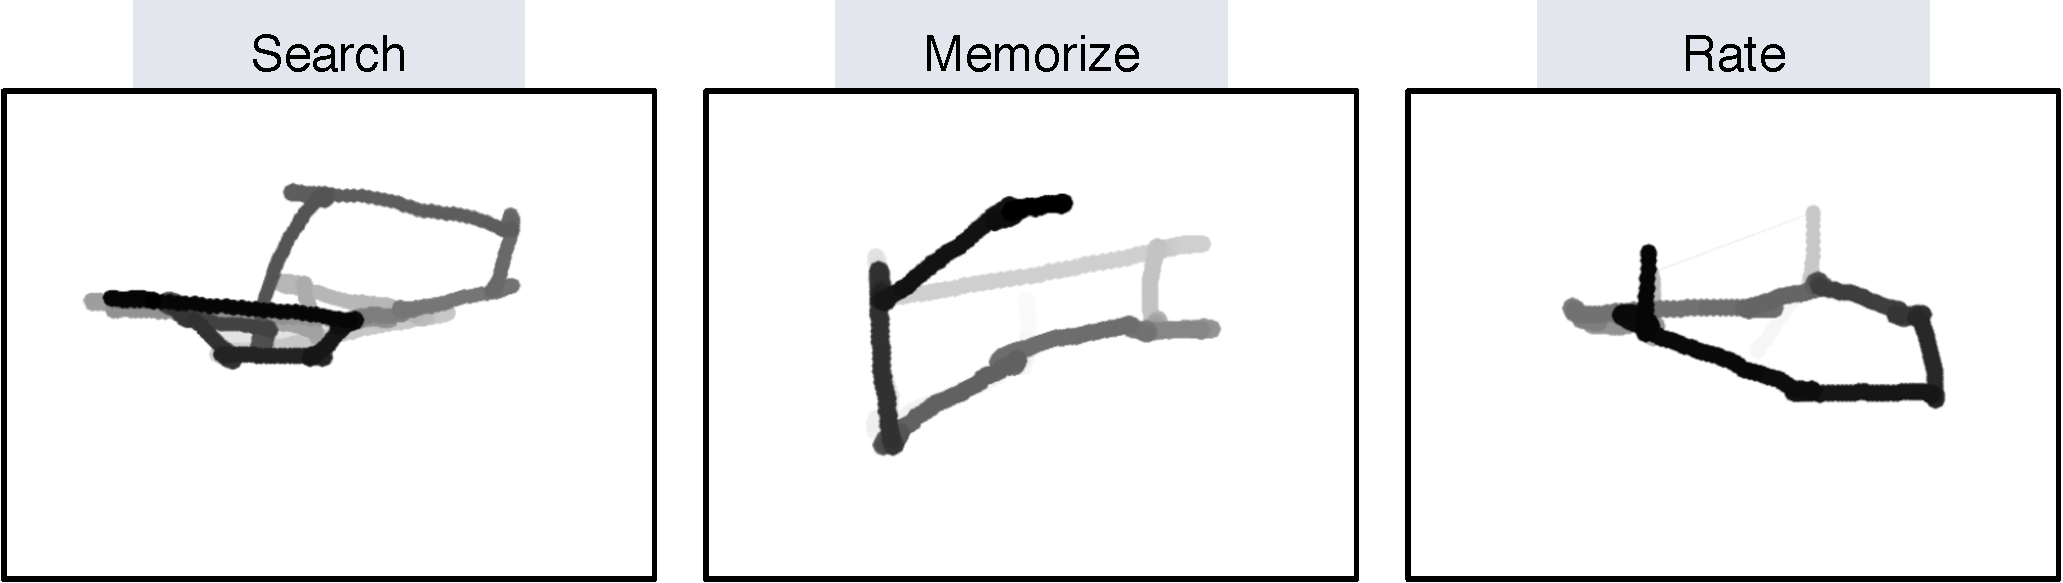
\includegraphics{figures/cond_imgs.pdf}
\caption{\label{fig:ave-condition}Each trial was represented as an image. Each sample collected within the trial was plotted as a dot in the image. Pupil size was represented by the size of the dot. The time course of the eye movements was represented by the gradual darkening of the dot over time.}
\end{figure}

\subsubsection{Data Subsets.}

The full timeline dataset was structured into three columns representing the x- and y- coordinates, and pupil size for each data point collected in the first six seconds of each trial. To systematically assess the predictive value of each XYP (i.e., x-coordinates, y-coordinates, pupil size) component of the data, the timeline and image datasets were batched into subsets that excluded one of the components (i.e., XY\(\varnothing\), X\(\varnothing\)P, \(\varnothing\)YP), or contained only one of the components (i.e., X\(\varnothing\varnothing\), \(\varnothing\)Y\(\varnothing\), \(\varnothing\varnothing\)P). For the timeline datasets, this means that the columns to be excluded in each data subset were replaced with zeros. The data were replaced with zeros because removing the columns would change the structure of the data. The same systematic batching process was carried out for the image dataset. See Figure \ref{fig:ave-subset} for an example of each of these image data subsets.



\begin{figure}
\centering
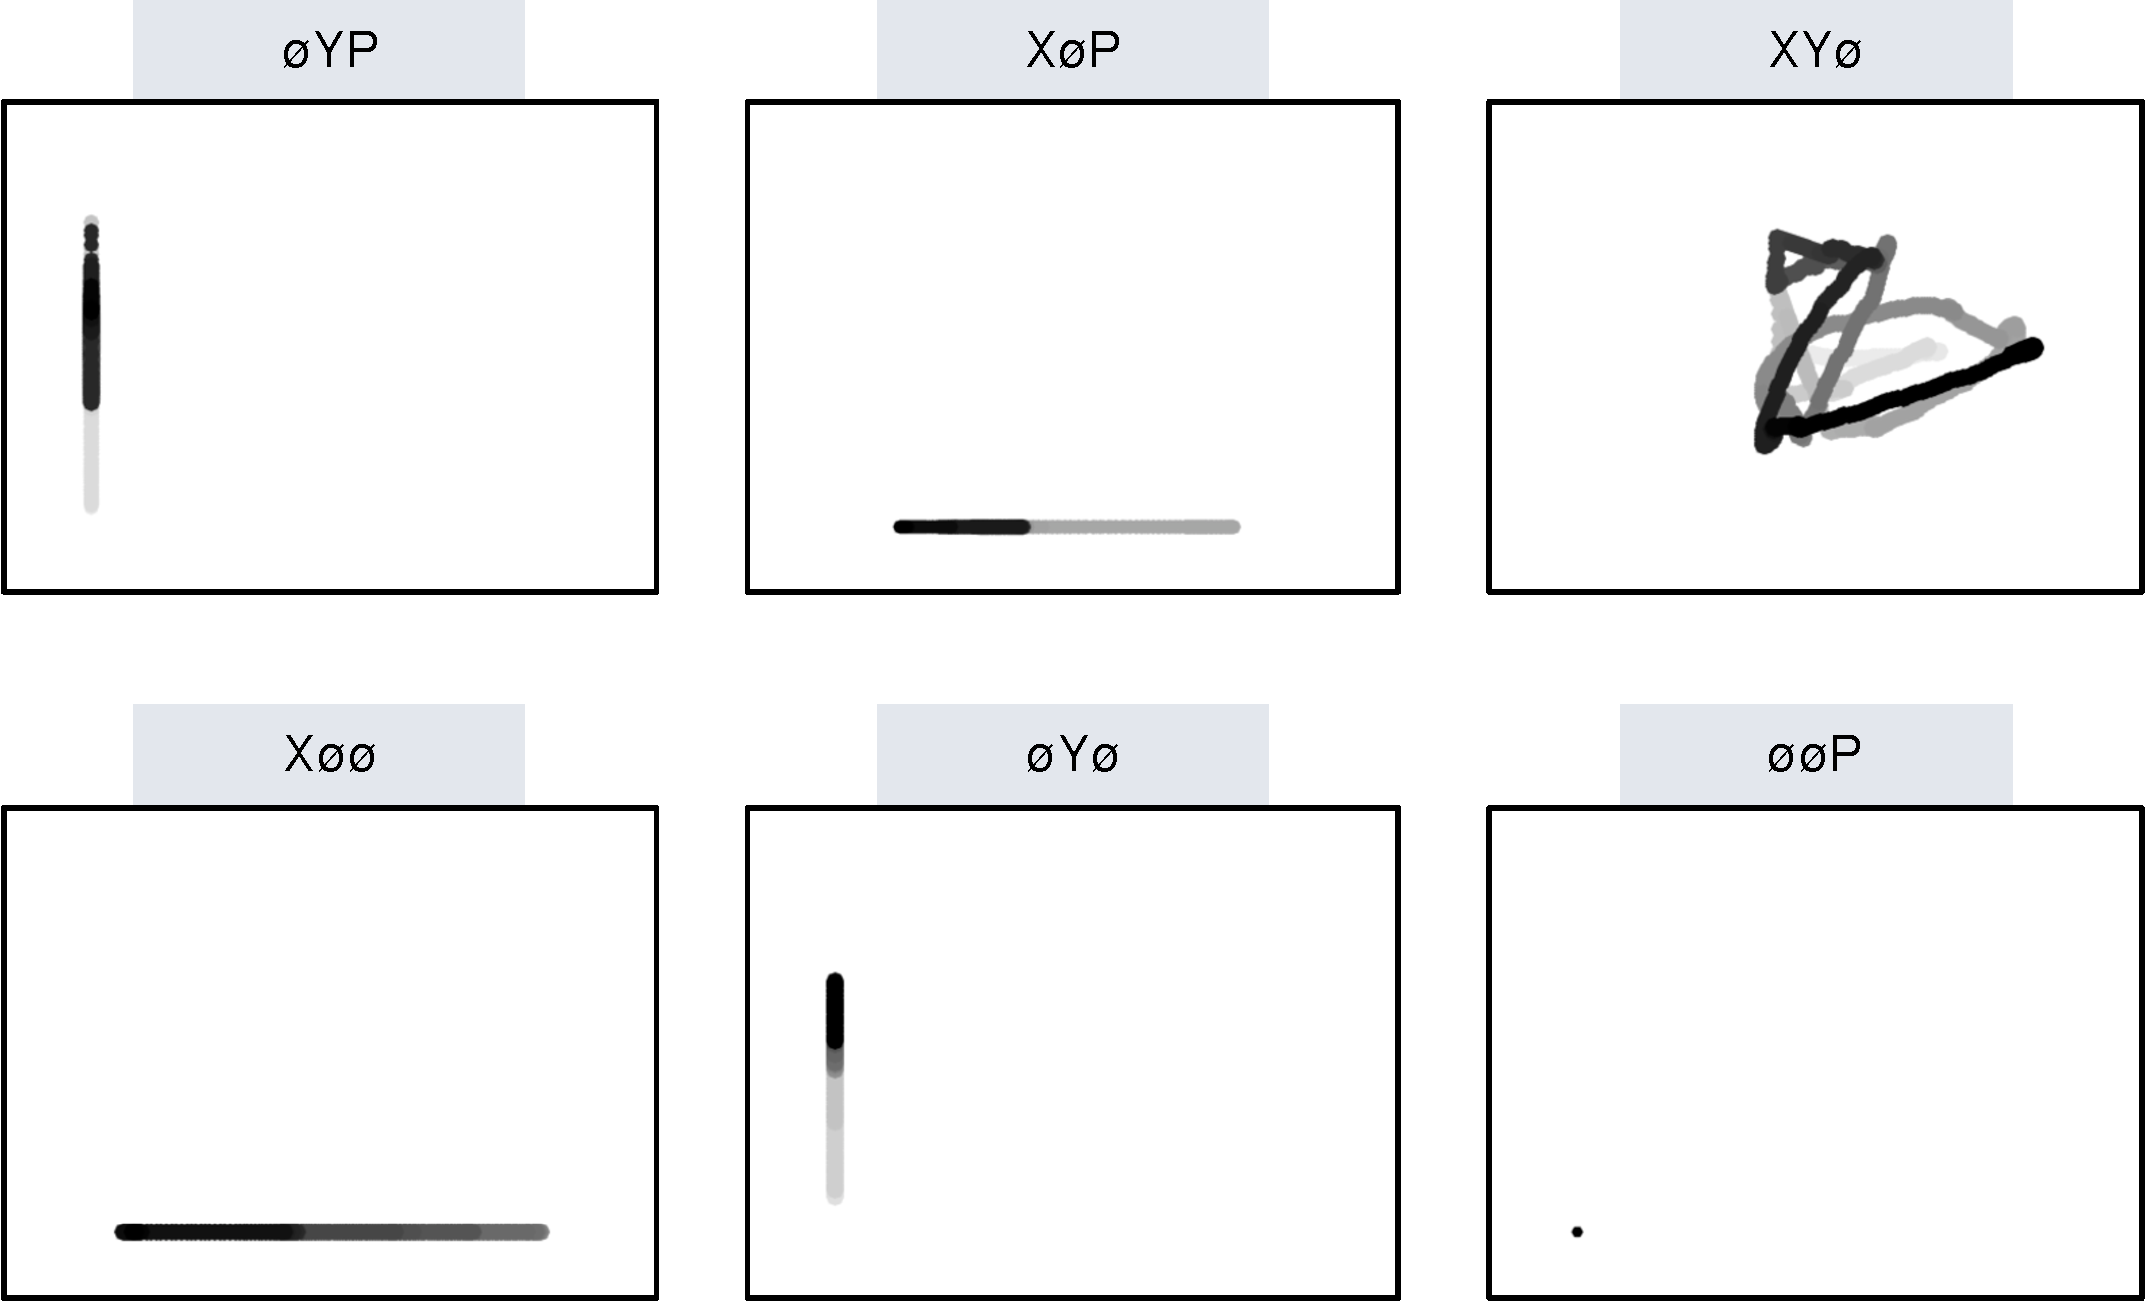
\includegraphics{figures/subset_imgs.pdf}
\caption{\label{fig:ave-subset}Plot images were used to represent data subsets that excluded one component of the eye movement data (i.e., XY\(\varnothing\), X\(\varnothing\)P, \(\varnothing\)YP) or contained only one component (i.e., X\(\varnothing\varnothing\), \(\varnothing\)Y\(\varnothing\), \(\varnothing\varnothing\)P). As with the trials in the full XYP dataset, the time course of the eye movements was represented by the shading of the dot. The first sample of each trial was white, and the last sample was black.}
\end{figure}

\subsection{Classification}

Deep CNN model architectures were implemented to classify the trials into Search, Memorize, or Rate categories. Because CNNs act as a digital filter sensitive to the number of features in the data, the differences in the structure of the timeline and image data formats necessitated separate CNN model architectures. The model architectures were developed with the intent of establishing a generalizable approach to classifying \textcolor{red}{task} from eye movement data.

The development of these models was not guided by any formal theoretical assumptions regarding the patterns or features likely to be extracted by the classifier. Like many HCI models, the development of these models followed general intuitions concerned with building a model architecture capable of transforming the data inputs into an interpretable feature set that would not overfit the dataset. The models were developed using version 0.3b of the DeLINEATE toolbox, which operates over a Keras backend (\url{http://delineate.it}; Kuntzelman et al., \textcolor{red}{in press}). Each training/test iteration randomly split the data so that 70\% of the trials were allocated to training, 15\% to validation, and 15\% to testing. \textcolor{red}{(This approach achieves essentially the same benefit of a more traditional k-fold cross-validation approach insofar as it allows all data to be used as both training and test without double-dipping; however, by resampling the data instead of using strict fold divisions, we can sidestep the issue of how to incorporate a validation set into the k-fold approach.)} Training of the model was stopped when validation accuracy did not improve over the span of 100 epochs. Once the early stopping threshold was reached, the resulting model was tested on the held-out test data. This process was repeated 10 times for each model, resulting in 10 classification accuracy scores for each model. The resulting accuracy scores were used for the comparisons against chance and other datasets or data subsets.

The models were developed and tested on the Exploratory dataset. Model hyperparameters were adjusted until the classification accuracies \textcolor{red}{on the test data appeared to peak, with no obvious evidence of excessive overfitting during the training process}. The model architecture with the highest classification accuracy on the Exploratory dataset was trained, validated, and tested independently on the Confirmatory dataset. This means that the model that was used to analyze the Confirmatory dataset was not trained on the Exploratory dataset. \textcolor{red}{For all of the analyses that excluded one or more components of the eye movement data (e.g., XY$\varnothing$, X$\varnothing$P, $\varnothing$YP, and so on), new models were trained for each data subset (i.e., data subset analyses did not use the model that had already been trained on the full XYP dataset).} The model architectures used for the timeline and plot image datasets are shown in Figure \ref{fig:models}\textcolor{red}{, with some additional details on the architecture hyperparameters in the figure caption}.



\begin{figure}
\centering
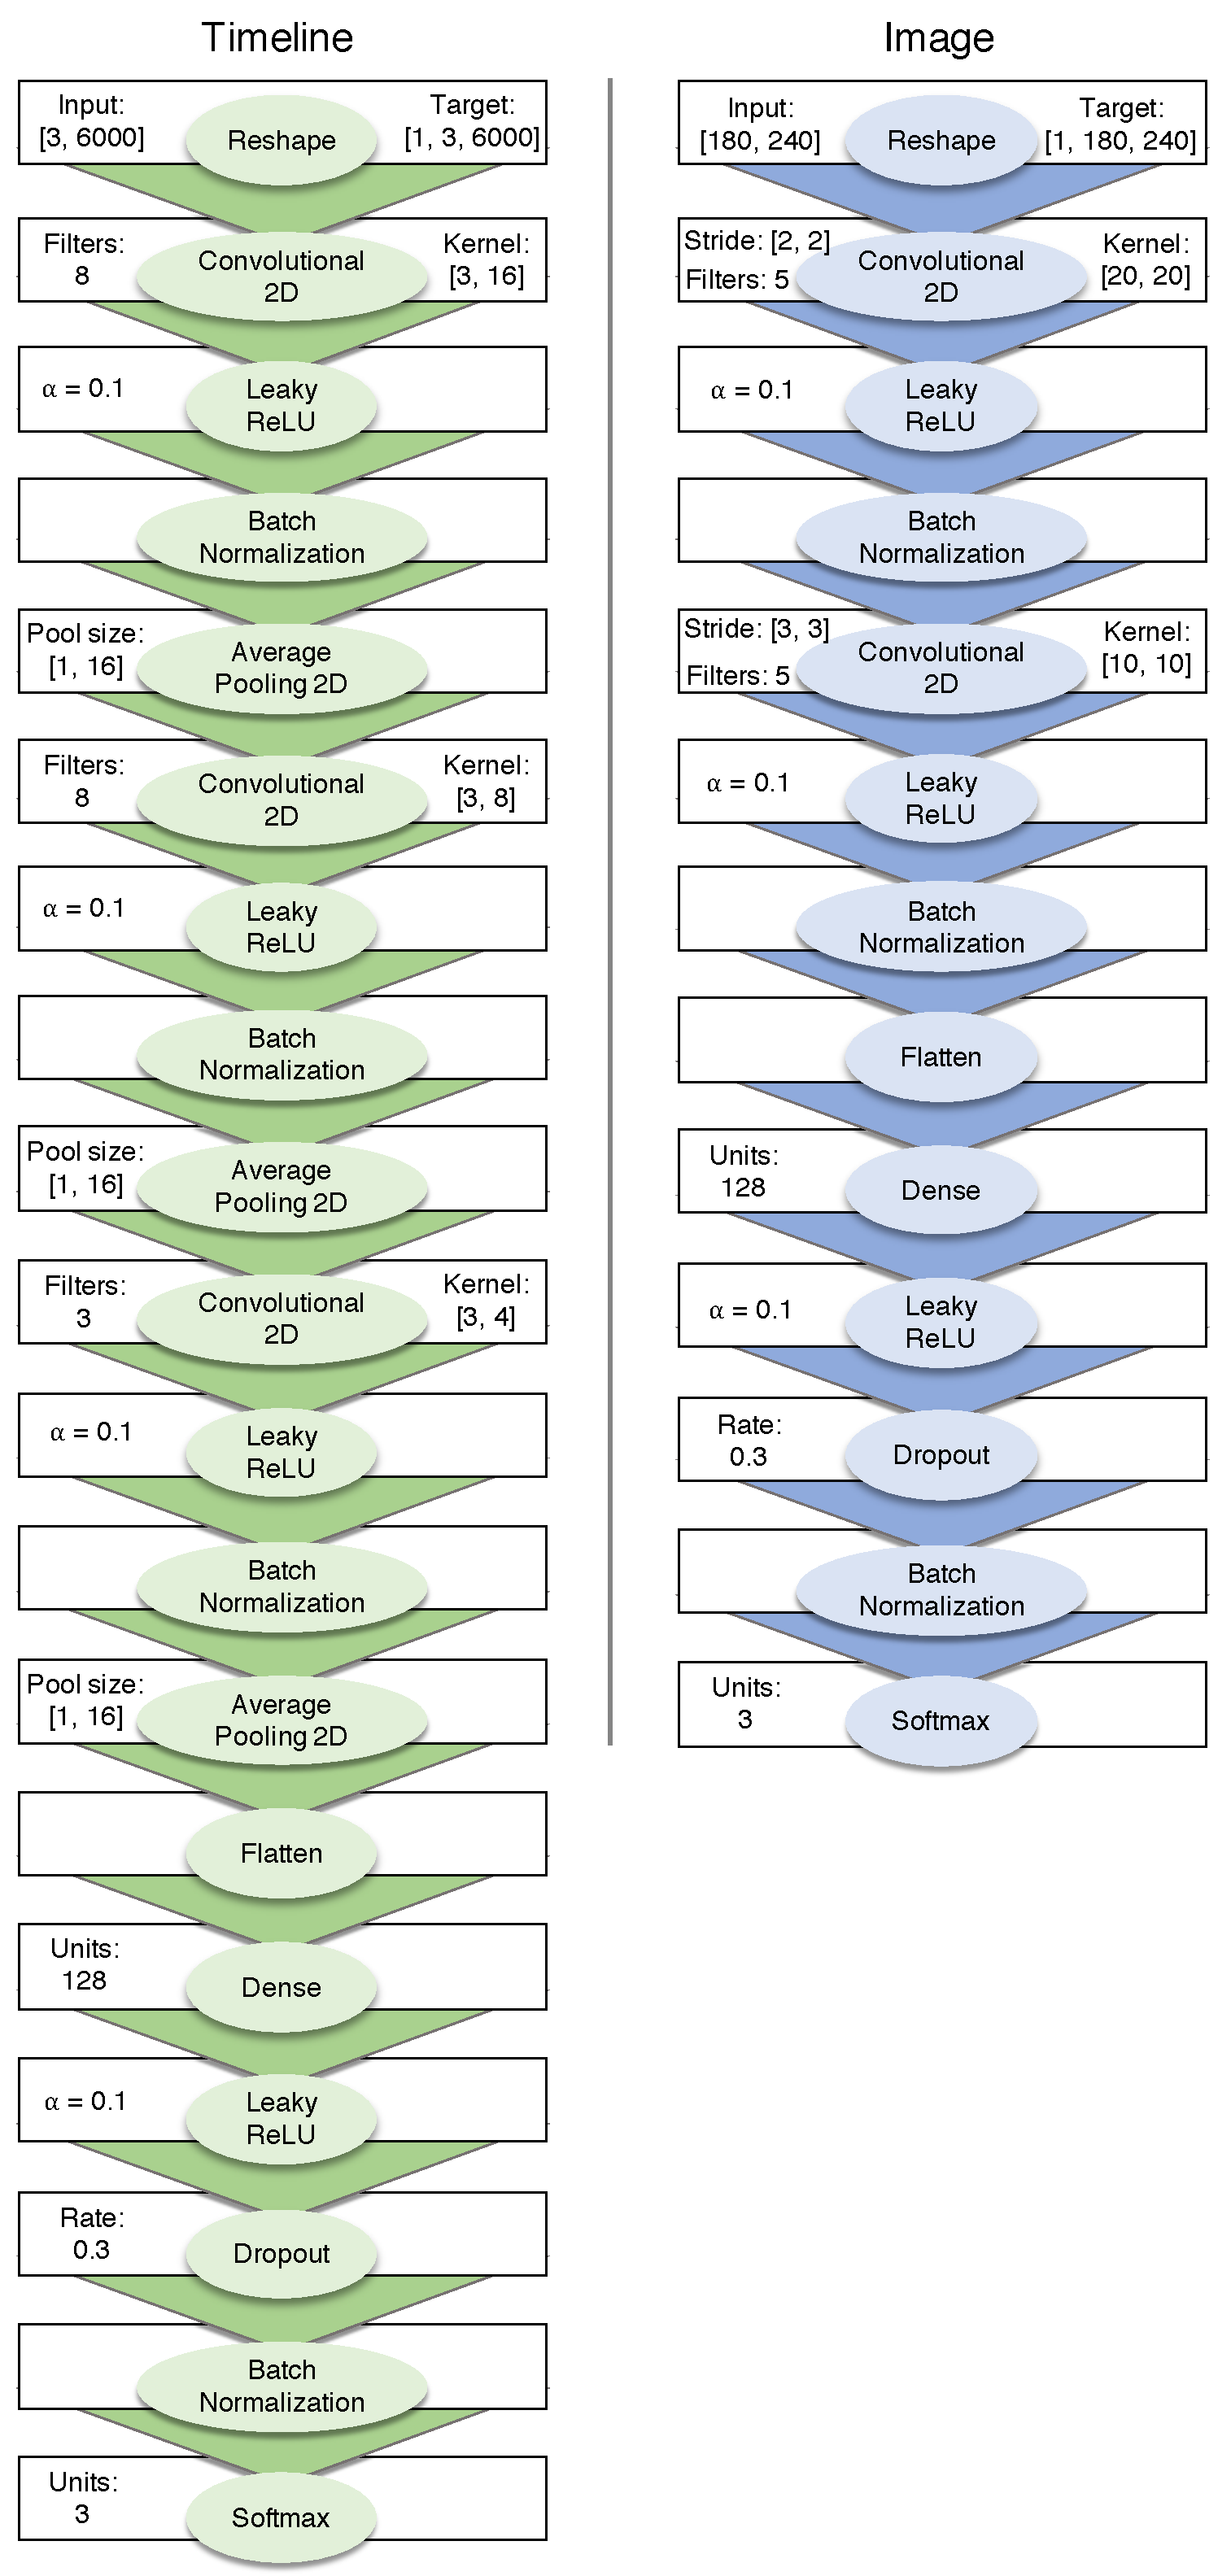
\includegraphics{figures/models.pdf}
\caption{\label{fig:models}Two different model architectures were used to classify the timeline and image data. Both models were compiled using a categorical crossentropy loss function, and optimized with the Adam algorithm. \textcolor{red}{Optimizer parameters were initial learning rate = 0.005, $\beta$$_1$ = 0.9, $\beta$$_2$ = 0.999, $\epsilon$ = 0.1. The timeline model had 16,946 trainable parameters (29,998 total); the image model had 18,525 trainable parameters (18,827 total).}}
\end{figure}

\subsection{Analysis}

Results for the CNN architecture that resulted in the highest accuracy on the Exploratory dataset are reported below. For every dataset tested, a one-sample two-tailed \emph{t}-test was used to compare the CNN accuracies against chance (33\%). The Shapiro-Wilk test was used to assess the normality for each dataset. When normality was assumed, the mean accuracy for that dataset was compared against chance using Student's one-sample two-tailed \emph{t}-test. When normality could not be assumed, the median accuracy for that dataset was compared against chance using Wilcoxon's Signed Rank test.

To determine the \textcolor{red}{independent contributions} of the three components of the eye movement data, the data subsets were compared within the timeline and plot image data types. If classification accuracies were lower when the data were batched into subsets, the component that was removed was assumed to have some unique contribution that the model was using to inform classification decisions. To determine the \textcolor{red}{uniqueness} of the contribution from each component, the accuracies from each subset with one component of the data removed were compared to the accuracies for the full dataset (XYP) using a one-way between-subjects Analysis of Variance (ANOVA). To further evaluate the decodability of each component independently, the accuracies from each subset containing only one component of the eye movement data were compared within a separate one-way between-subjects ANOVA. All post-hoc comparisons were corrected using Tukey's HSD.

\section{Results}
\subsection{Timeline Data Classification}
\subsubsection{Exploratory.}

Classification accuracies for the XYP timeline dataset were well above chance (chance = .33; \emph{M} = .526, \emph{SD} = .018; \emph{t}\(_{9}\) = 34.565, \emph{p} \textless{} .001). Accuracies for classifications of the batched data subsets were all better than chance (see Figure \ref{fig:timeline-parcellation-chance}). As shown in the confusion matrices displayed in Figure \ref{fig:timeline-conf-matrices}, the data subsets with lower overall classification accuracies almost always classified the Memorize condition at or below chance levels of accuracy. Misclassifications of the Memorize condition were split relatively evenly between the Search and Rate conditions.

\begin{figure}
\centering
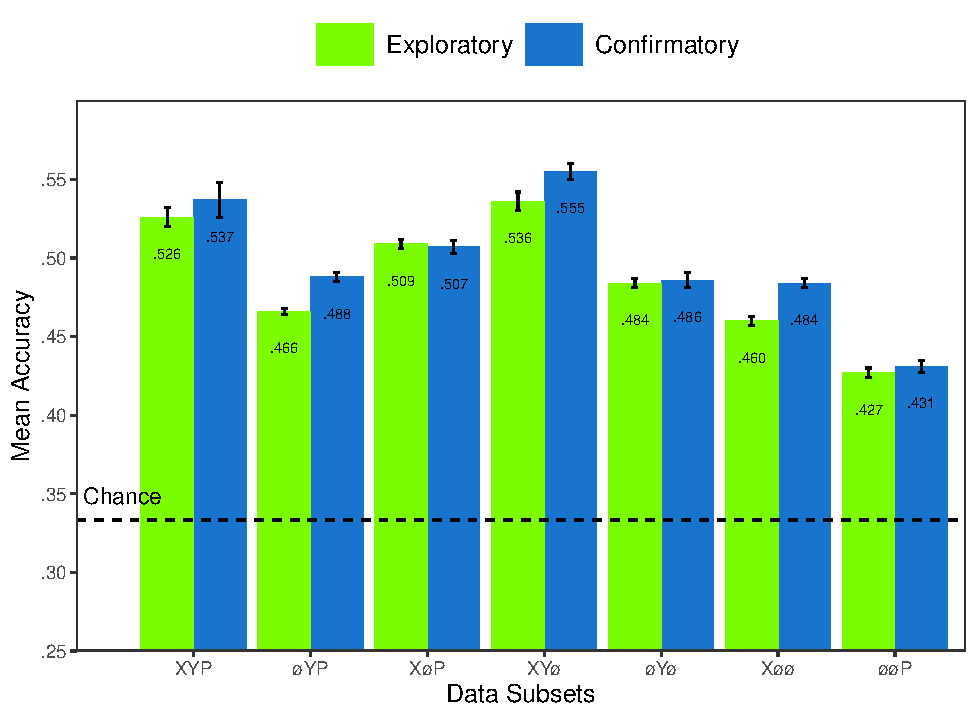
\includegraphics{figures/r_code/timeline_subset_chance.pdf}
\caption{\label{fig:timeline-parcellation-chance}All of the data subsets were decoded at levels better than chance (.33). Each subset is labeled with the mean accuracy. The error bars represent standard errors.}
\end{figure}

\begin{figure}
\centering
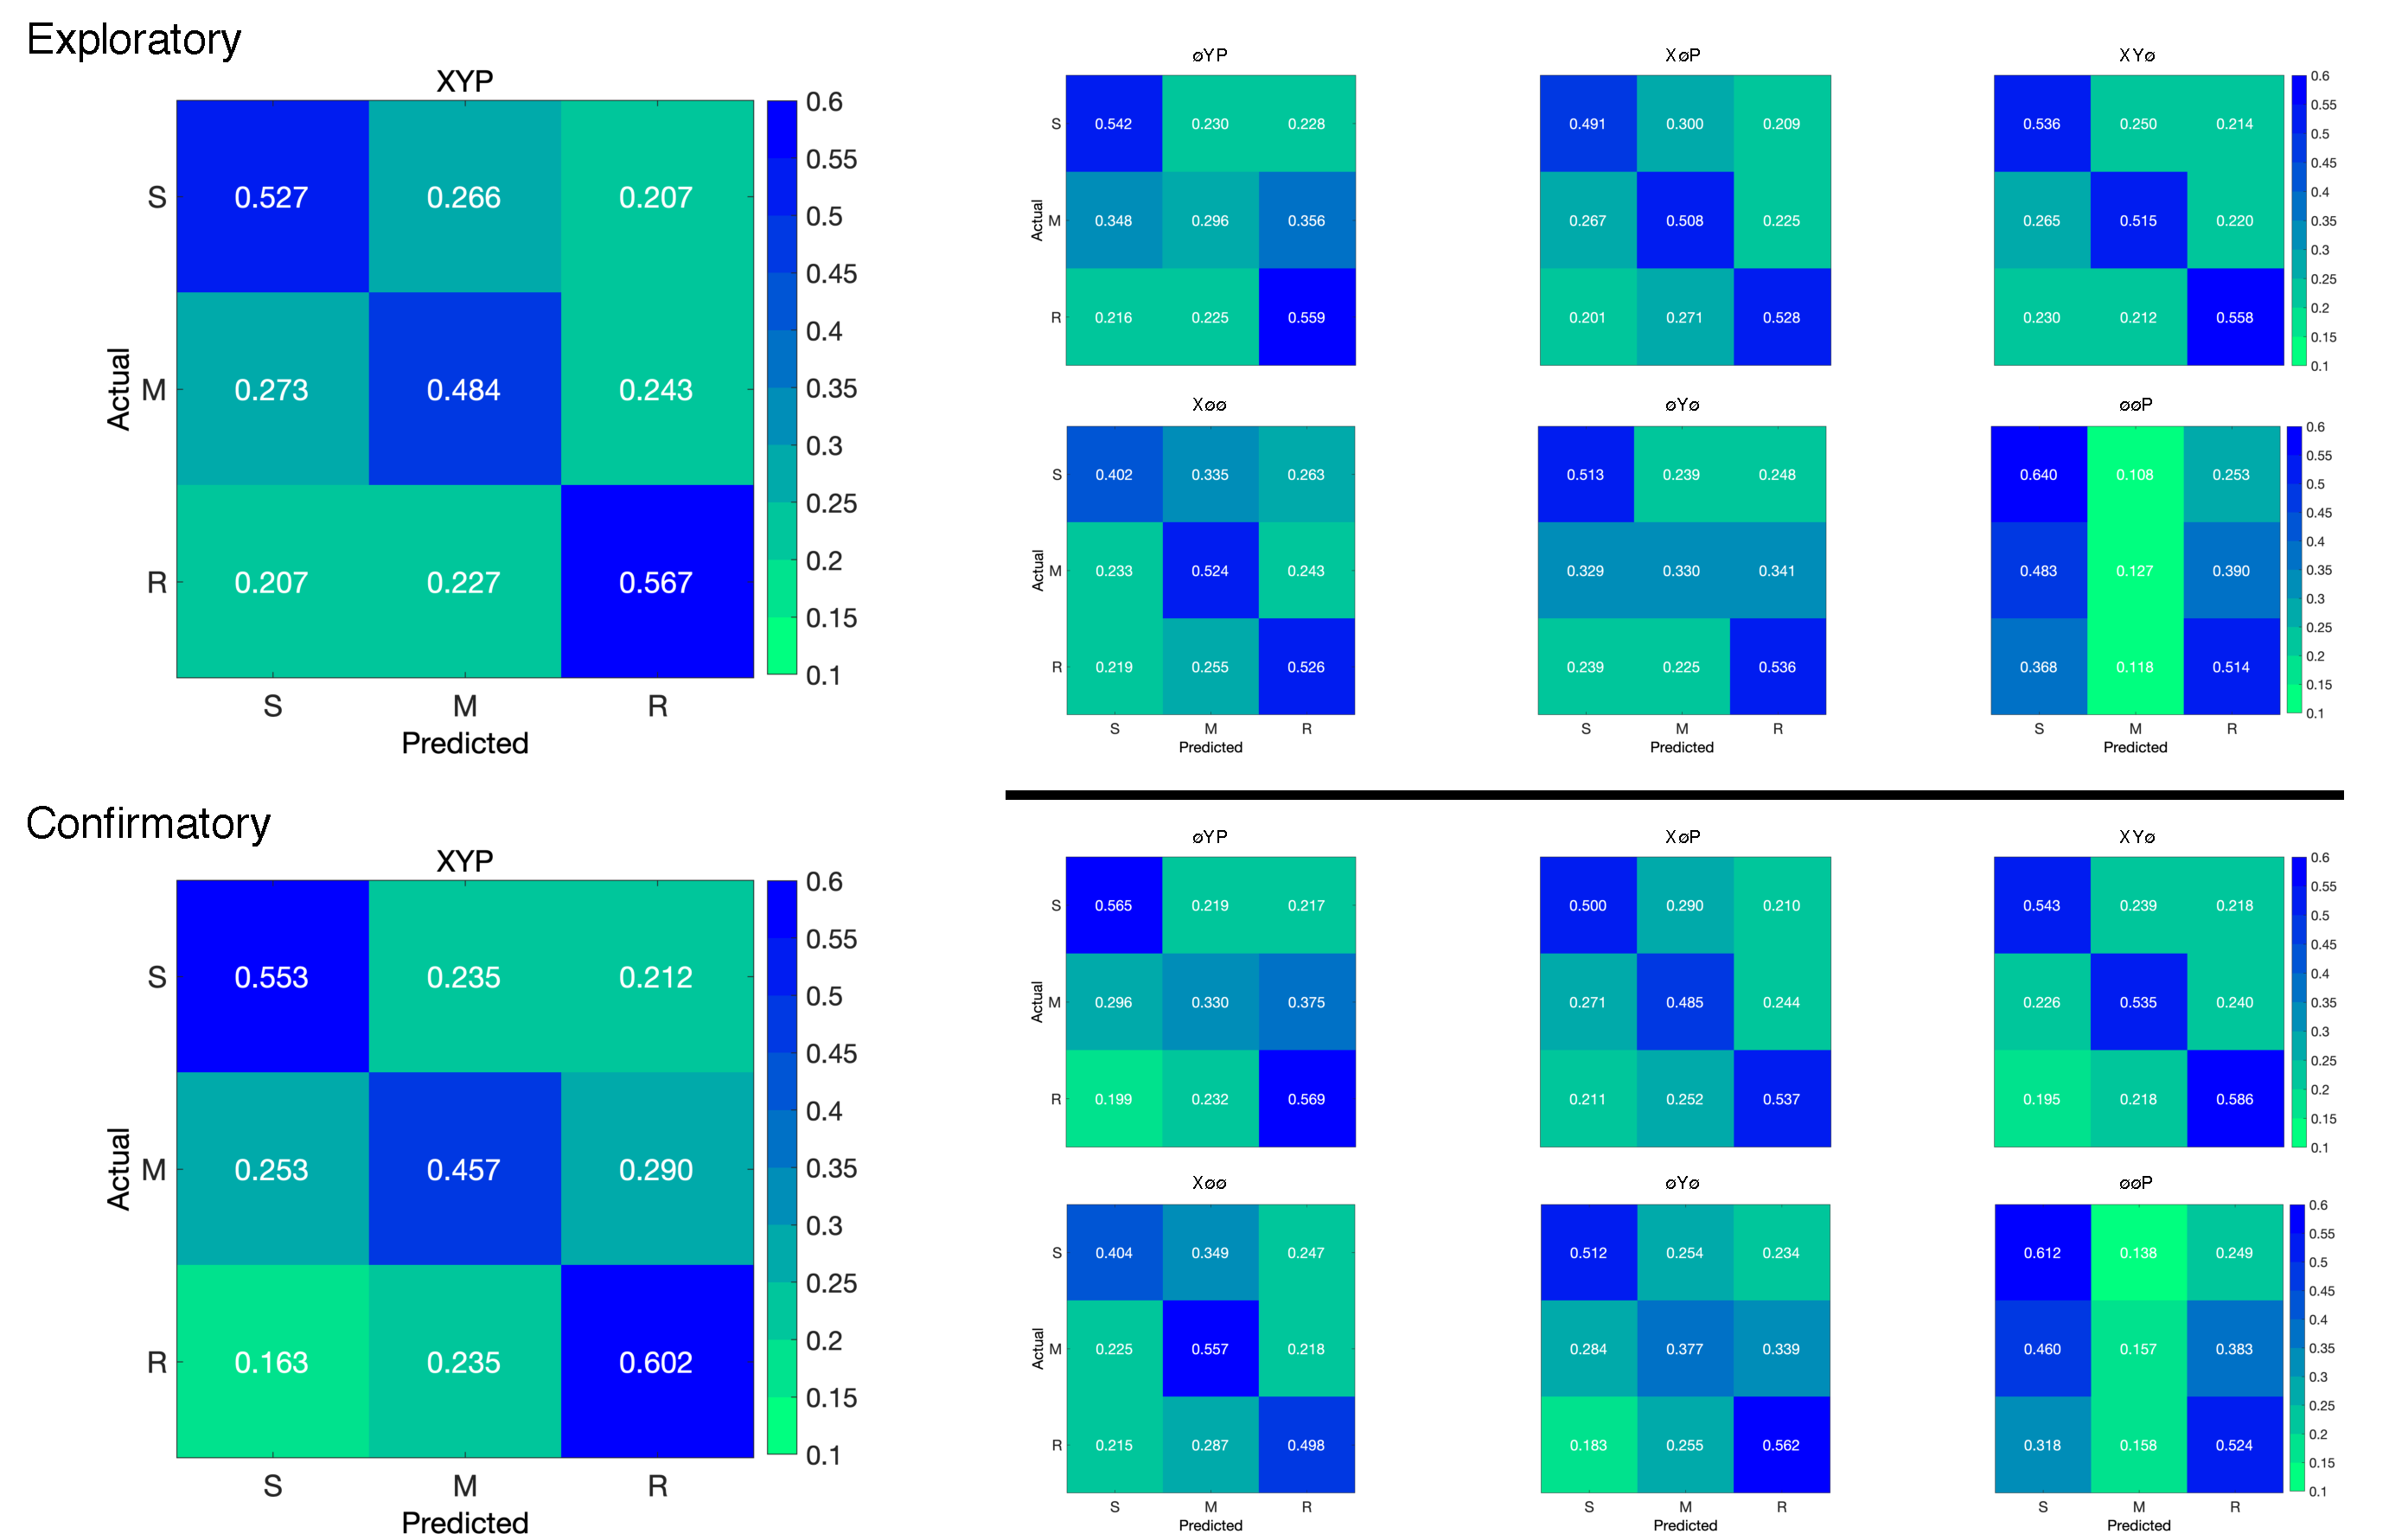
\includegraphics{figures/timeline_conf_matrices.pdf}
\caption{\label{fig:timeline-conf-matrices}The confusion matrices represent the average classification accuracies for each condition of the timeline data (S = Search, M = Memorize, R = Rate). The vertical axis of the confusion matrices represents the actual condition for the trial. The horizontal axis of the confusion matrices represents the condition that was predicted by the model.}
\end{figure}

There was a difference in classification accuracy for the XYP dataset and the subsets that had the pupil size, x-coordinate, and y-coordinate data systematically removed (\emph{F}\(_{3, 36}\) = 47.471, \emph{p} \textless{} .001, \textit{$\eta$}\(^{2}\) = 0.798). Post-hoc comparisons against the XYP dataset showed that classification accuracies were not affected by the removal of pupil size or y-coordinate data (see Table \ref{tab:timeline-parcellation-comparisons}). The null effect present when pupil size was removed suggests that the pupil size data were not contributing unique information that was not otherwise provided by the x- and y-coordinates. A strict significance threshold of \(\alpha\) = .05 implies the same conclusion for the y-coordinate data, but the relatively low degrees of freedom (\emph{df} = 18) and the borderline observed \emph{p}-value (\emph{p} = .056) afford the possibility that there exists a small effect. However, classification for the \(\varnothing\)YP subset was significantly lower than the XYP dataset, showing that the x-coordinate data were uniquely informative to the classification.

\begin{table}[!h]
    \centering
    \caption{Timeline Subset Comparisons}
    \label{tab:timeline-parcellation-comparisons}
    \begin{tabular}{l c c c c}
         & \multicolumn{2}{c}{Exploratory} & \multicolumn{2}{c}{Confirmatory} \\
        \hline
        Comparison & \textit{t} & \multicolumn{1}{c|}{\textit{p}} & \textit{t} & \textit{p} \\
        \hline
        XYP vs. $\varnothing$YP & 9.420 & \multicolumn{1}{c|}{< .001} & 5.210 & < .001 \\
        XYP vs. X$\varnothing$P & 2.645 & \multicolumn{1}{c|}{.056} & 3.165 & .016 \\
        XYP vs. XY$\varnothing$ & 1.635 & \multicolumn{1}{c|}{.372} & 1.805 & .288 \\
        X$\varnothing\varnothing$ vs. $\varnothing$Y$\varnothing$ & 5.187 & \multicolumn{1}{c|}{< .001} & 0.495 & .874 \\
        X$\varnothing\varnothing$ vs. $\varnothing\varnothing$P & 12.213 & \multicolumn{1}{c|}{< .001} & 10.178 & < .001 \\
        $\varnothing$Y$\varnothing$ vs. $\varnothing\varnothing$P & 7.026 & \multicolumn{1}{c|}{< .001} & 9.683 & < .001 \\
        \hline
    \end{tabular}
\end{table}

There was also a difference in classification accuracies for the X\(\varnothing\varnothing\), \(\varnothing\)Y\(\varnothing\), and \(\varnothing\varnothing\)P subsets (\emph{F}\(_{2, 27}\) = 75.145, \emph{p} \textless{} .001, \textit{$\eta$}\(^{2}\) = 0.848). Post-hoc comparisons showed that classification accuracy for the \(\varnothing\varnothing\)P subset was lower than the X\(\varnothing\varnothing\) and \(\varnothing\)Y\(\varnothing\) subsets. Classification accuracy for the X\(\varnothing\varnothing\) subset was higher than the \(\varnothing\)Y\(\varnothing\) subset. Altogether, these findings suggest that pupil size data was the least uniquely informative to classification decisions, while the x-coordinate data was the most uniquely informative.

\subsubsection{Confirmatory.}

Classification accuracies for the Confirmatory XYP timeline dataset were well above chance (\emph{M} = .537, \emph{SD} = 0.036, \emph{t}\(_{9}\) = 17.849, \emph{p} \textless{} .001). Classification accuracies for the data subsets were also better than chance (see Figure \ref{fig:timeline-parcellation-chance}). Overall, there was high similarity in the pattern of results for the Exploratory and Confirmatory datasets (see Figure \ref{fig:timeline-parcellation-chance}). Furthermore, the general trend showing that pupil size was the least informative eye tracking data component was replicated in the Confirmatory dataset (see Table \ref{tab:timeline-parcellation-comparisons}). Also in concordance with the Exploratory timeline dataset, the confusion matrices for these data revealed that the Memorize task was mis-classified more often than the Search and Rate tasks (see Figure \ref{fig:timeline-conf-matrices}).

To test the generalizability of the model architecture, classification accuracies for the XYP Exploratory and Confirmatory timeline datasets were compared. The Shapiro-Wilk test for normality indicated that the Exploratory (\emph{W} = 0.937, \emph{p} = .524) and Confirmatory (\emph{W} = 0.884, \emph{p} = .145) datasets were normally distributed, but Levene's test indicated that the variances were not equal, \emph{F}\(_{1, 18}\) = 8.783, \emph{p} = .008. Welch's unequal variances \emph{t}-test did not show a difference between the two datasets, \emph{t}\(_{13.045}\) = 0.907, \emph{p} = .381, Cohen's \emph{d} = 0.406. These findings indicate that the deep learning model decoded the Exploratory and Confirmatory timeline datasets equally well, but the Confirmatory dataset classifications were less consistent across training/test iterations (as indicated by the increase in standard deviation).

\subsection{Plot Image Classification}
\subsubsection{Exploratory.}

Classification accuracies for the XYP plot image data were better than chance (\emph{M} = .436, \emph{SD} = .020, \emph{p} \textless{} .001), but were less accurate than the classifications for the XYP Exploratory timeline data (\emph{t}\(_{18}\) = 10.813, \emph{p} \textless{} .001). Accuracies for the classifications for all subsets of the plot image data except the \(\varnothing\varnothing\)P subset were better than chance (see Figure \ref{fig:img-parcellation-chance}). Following the pattern expressed by the timeline dataset, the confusion matrices showed that the Memorize condition was misclassified more often than the other conditions, and appeared to be equally mis-identified as a Search or Rate condition (see Figure \ref{fig:img-conf-matrices}).

\begin{figure}
\centering
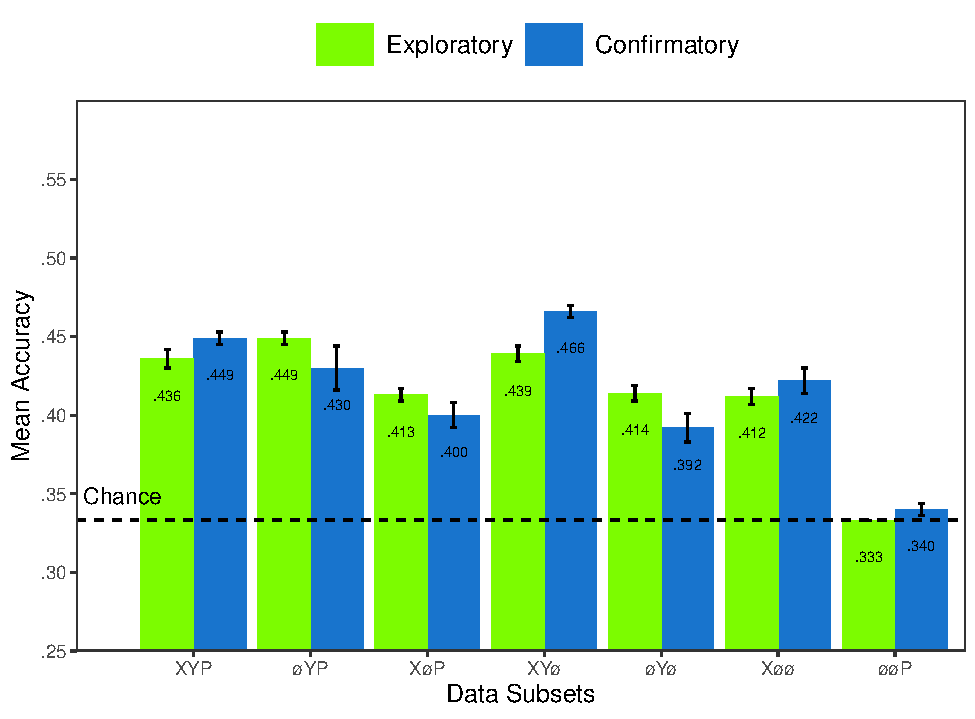
\includegraphics{figures/r_code/img_subset_chance.pdf}
\caption{\label{fig:img-parcellation-chance}All of the data subsets except for the Exploratory \(\varnothing\varnothing\)P dataset were decoded at levels better than chance (.33). Each subset is labeled with the mean accuracy. The error bars represent standard errors.}
\end{figure}

\begin{figure}
\centering
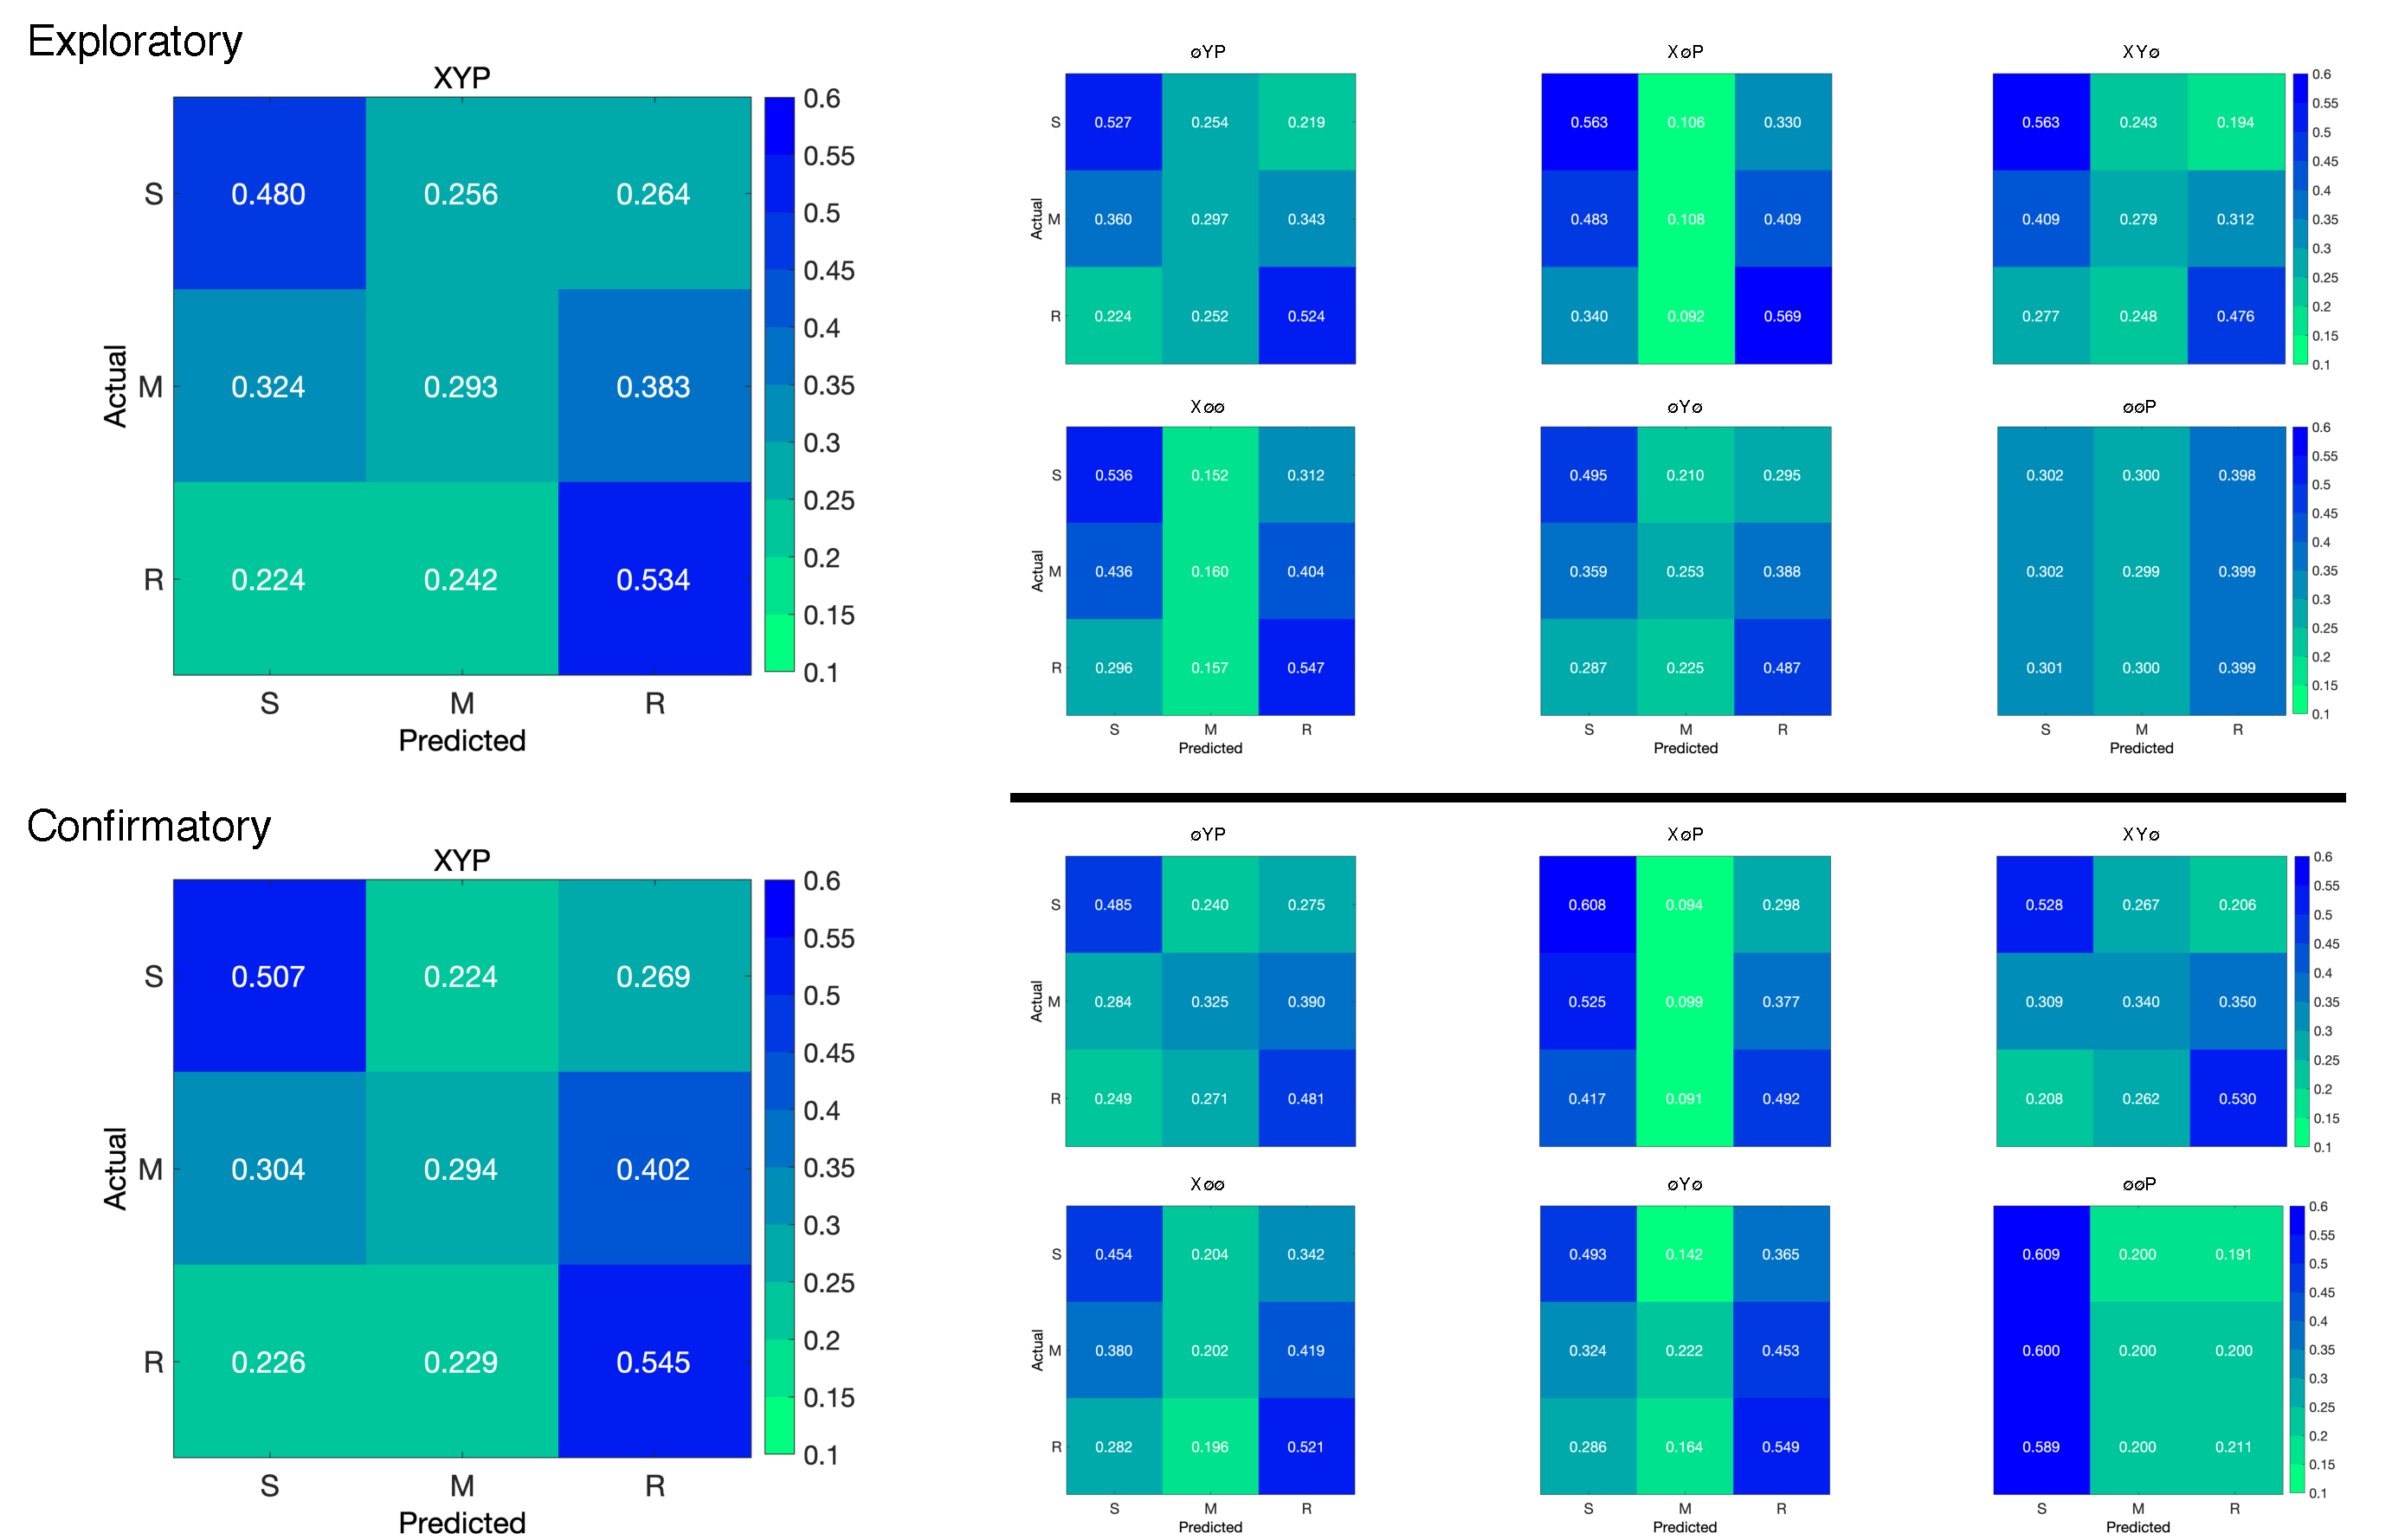
\includegraphics{figures/img_conf_matrices.pdf}
\caption{\label{fig:img-conf-matrices}The confusion matrices represent the average classification accuracies for each condition of the image data (S = Search, M = Memorize, R = Rate). The vertical axis of the confusion matrices represents the actual condition for the trial. The horizontal axis of the confusion matrices represents the condition that was predicted by the model.}
\end{figure}

There was a difference in classification accuracy between the XYP dataset and the data subsets (\emph{F}\(_{4, 45}\) = 7.093, \emph{p} \textless{} .001, \textit{$\eta$}\(^{2}\) = .387). Post-hoc comparisons showed that compared to the XYP dataset, there was no effect of removing pupil size or the x-coordinates, but classification accuracy was worse when the y-coordinates were removed (see Table \ref{tab:image-parcellation-comparisons}).

\begin{table}[!h]
    \centering
    \caption{Image Subset Comparisons}
    \label{tab:image-parcellation-comparisons}
    \begin{tabular}{l c c c c}
         & \multicolumn{2}{c}{Exploratory} & \multicolumn{2}{c}{Confirmatory} \\
        \hline
        Comparison & \textit{t} & \multicolumn{1}{c|}{\textit{p}} & \textit{t} & \textit{p} \\
        \hline
        XYP vs. $\varnothing$YP & 1.792 & \multicolumn{1}{c|}{.391} & 1.623 & .491 \\
        XYP vs. X$\varnothing$P & 2.939 & \multicolumn{1}{c|}{.039} & 4.375 & < .001 \\
        XYP vs. XY$\varnothing$ & 0.474 & \multicolumn{1}{c|}{.989} & 1.557 & .532 \\
        X$\varnothing\varnothing$ vs. $\varnothing$Y$\varnothing$ & 0.423 & \multicolumn{1}{c|}{.906} & 2.807 & .204 \\
        X$\varnothing\varnothing$ vs. $\varnothing\varnothing$P & 13.569 & \multicolumn{1}{c|}{< .001} & 5.070 & < .001 \\
        $\varnothing$Y$\varnothing$ vs. $\varnothing\varnothing$P & 13.235 & \multicolumn{1}{c|}{< .001} & 7.877 & < .001 \\
        \hline
    \end{tabular}
\end{table}

There was also a difference in classification accuracies between the X\(\varnothing\varnothing\), \(\varnothing\)Y\(\varnothing\), and \(\varnothing\varnothing\)P subsets (Levene's test: \emph{F}\(_{2, 27}\) = 3.815, \emph{p} = .035; Welch correction for lack of homogeneity of variances: \emph{F}\(_{2, 17.993}\) = 228.137, \emph{p} \textless{} .001, \textit{$\eta$}\(^{2}\) = .899). Post-hoc comparisons showed that there was no difference in classification accuracies for the X\(\varnothing\varnothing\) and \(\varnothing\)Y\(\varnothing\) subsets, but classification for the \(\varnothing\varnothing\)P subset were less accurate than the X\(\varnothing\varnothing\) and \(\varnothing\)Y\(\varnothing\) subsets.

\subsubsection{Confirmatory.}

Classification accuracies for the XYP confirmatory image dataset were well above chance (\emph{M} = .449, \emph{SD} = 0.012, \emph{t}\(_{9}\) = 31.061, \emph{p} \textless{} .001), but were less accurate than the classifications of the confirmatory timeline dataset (\emph{t}\(_{18}\) = 11.167, \emph{p} \textless{} .001). Accuracies for classifications of the data subsets were also all better than chance (see Figure \ref{fig:img-parcellation-chance}). The confusion matrices followed the pattern showing that the Memorize condition was mistaken most often, and was relatively equally mis-identified as a Search or Rate trial (see Figure \ref{fig:img-conf-matrices}). As with the timeline data, the general trend showing that pupil size data was the least informative to the model was replicated in the Confirmatory dataset (see Table \ref{tab:image-parcellation-comparisons}).

To test the generalizability of the model architecture, the classification accuracies for the XYP Exploratory and Confirmatory plot image datasets were compared. The independent samples \emph{t}-test comparing the classification accuracies for the Exploratory and Confirmatory plot image datasets did not show a significant difference, \emph{t}\(_{18}\) = 1.777, \emph{p} = .092, Cohen's \emph{d} = 0.795.

\section{Discussion}

The present study aimed to produce a practical and reliable example of a black box solution to the inverse Yarbus problem. To implement this solution, we classified raw timeline and minimally processed plot image data using a CNN model architecture. To our knowledge, this study was the first to provide a solution to determining \textcolor{red}{task} from eye movement data using each of the following: (1) Non-aggregated eye tracking data (i.e., raw x-coordinates, y-coordinates, pupil size), (2) timeline and image data formats (see Figure \ref{fig:ave-subset}), and (3) a black box CNN architecture. This study probed the \textcolor{red}{independent contributions} of the x-coordinate, y-coordinate, and pupil size components of the eye movement data using a CNN. The CNN was able to decode the timeline and plot image data better than chance, although only the timeline datasets were decoded with accuracies comparable to other state-of-the-art approaches. Datasets with lower classification accuracies were not able to differentiate the cognitive processes underlying the Memorize task from the cognitive processes underlying the Search and Rate tasks. Decoding subsets of the data revealed that pupil size was the least uniquely informative component of the eye movement data. This pattern of findings was consistent between the Exploratory and Confirmatory datasets.

Although several aggregate eye movement features have been tested as task predictors, to our knowledge, no other study has assessed the predictive value of the data format (viz., data in the format of a plot image). Our results suggest that although CNNs are robust image classifiers, eye movement data is decoded in the standard timeline format more effectively than in image format. This may be because the image data format contains less decodable information than the timeline format. Over the span of the trial (six seconds), the eye movements occasionally overlapped. When there was an overlap in the image data format, the more recent data points overwrote the older data points. This resulted in some information loss that did not occur when the data were represented in the raw timeline format. Despite this loss of information, the plot image format was still decoded with better than chance accuracy. To further examine the viability of classifying task from eye movement image datasets, future research might consider representing the data in different forms such as 3-dimensional data formats, or more complex color combinations capable of representing overlapping data points.

When considering the superior performance of the timeline data (vs., plot image data), we must also consider the differences in the model architectures. Because the structures of the timeline and plot image data formats were different, the models decoding those data structures also needed to be different. Both model architectures were optimized individually on the Exploratory dataset before being tested on the Confirmatory dataset. For both timeline and plot image formats, there was good replicability between the Exploratory and Confirmatory datasets, demonstrating that these architectures performed similarly from experiment to experiment. An appropriately tuned CNN should be capable of learning any arbitrary function, but given that the upper bound for decodability of these datasets is unknown, there is the possibility that a model architecture exists that is capable of classifying the plot image data format more accurately than the model used to classify the timeline data. Despite this possibility, the convergence of these findings with other studies (see Table \ref{tab:previous-studies}) suggests that the results of this study are approaching a ceiling for the potential to solve the inverse Yarbus problem with eye movement data. \textcolor{red}{We attempted to replicate some of those other studies' methods on our own dataset, but were only able to do so with the methods of }Coco and Keller (2014)\textcolor{red}{, due to lack of publicly available code or incompatibility with our data; for Coco and Keller's methods, we did not achieve better-than-chance classification in our data.} Although the true capacity to predict mental state from eye movement data is unknown, standardizing datasets in the future could provide a point for comparison that can more effectively indicate which methods are most effective at solving the inverse Yarbus problem. \textcolor{red}{As a gesture towards this goal, we have made the data and code from the present study publicly available at: INSERTLINKHERE.}

In the current study, the Memorize condition was classified less accurately than the Search and Rate conditions, especially for the datasets with lower overall accuracy. This suggests that the eye movements associated with the Memorize task were potentially lacking unique or informative features to decode. This means that eye movements associated with the Memorize condition were interpreted as noise, or were sharing features of underlying cognitive processes that were represented in the eye movements associated with the Search and Rate tasks. Previous research (e.g., Król \& Król, 2018) has attributed the inability to differentiate one condition from the others to the overlapping of sub-features in the eye movements between two tasks that are too subtle to be represented in the eye movement data.

To more clearly understand how the different tasks influenced the decodability of the eye movement data, additional analyses were conducted on the Exploratory and Confirmatory timeline datasets (see Appendix). For the main supplementary analysis, the data subsets were re-submitted to the CNN and re-classified as 2-category task sets. In addition to the main supplementary analysis, the results from the primary analysis were re-calculated from 3-category task sets to 2-category task sets. In the primary analyses, the Memorize condition was predicted with the lowest accuracy, but mis-classifications of the Search and Rate trials were most often categorized as Memorize. As a whole, this pattern of results and the main supplementary analysis indicated a general bias for uncertain trials to be categorized as Memorize. As expected, the main supplementary analysis also showed that the 2-category task set that included only Search and Rate had higher accuracies than both of the 2-category task sets that included the Memorize condition. The re-calculation analysis generally replicated the pattern of results seen in the main supplementary analysis but with larger variance, suggesting that including lower-accuracy trial types during model training can decrease the consistency of classifier performance. Overall, the findings from this supplemental analysis show that conclusions drawn from comparisons between approaches that do not use the same task sets, or the same number of tasks, could be potentially uninterpretable because the features underlying the task categories are interpreted differently by the neural network algorithm.

When determining the \textcolor{red}{unique} contributions of the the eye movement features used in this study (x-coordinates, y-coordinates, pupil size), the pupil size data was consistently the least uniquely informative. When pupil size was removed from the Exploratory and Confirmatory timeline and plot image datasets, classification accuracy remained stable (vs., XYP dataset). Furthermore, classification accuracy of the \(\varnothing\varnothing\)P subset was the lowest of all of the data subsets, and in one instance, was no better than chance. Although these findings indicate that, in this case, pupil size was a relatively uninformative component of the eye movement data, previous research has associated changes in pupil size as indicators of working memory load (Kahneman \& Beatty, 1966; Karatekin, Couperus, \& Marcus, 2004), arousal (Wang et al., 2018), and cognitive effort (Porter, Troscianko, \& Gilchrist, 2007). The results of the current study indicate that the changes in pupil size associated with these underlying processes were not useful in delineating the tasks being classified (i.e., Search, Memorize, Rate), potentially because these tasks did not evoke a reliable pattern of changes in pupil size. Additionally, properties of the stimuli known to influence pupil size, such as luminance and contrast, were not controlled in these datasets. Given that stimuli were randomly assigned, there is the possibility that uncontrolled stimulus properties known to affect pupil size impeded the CNN's capacity to detect patterns in the pupil size data.

The findings from the current study support the notion that black box CNNs are a viable approach to determining task from eye movement data. In a recent review, Lukander et al. (2017) expressed concern regarding the lack of generalizability of black box approaches when decoding eye movement data. Overall, the current study showed a consistent pattern of results for the XYP timeline and image datasets, but some minor inconsistencies in the pattern of results for the x- and y- coordinate subset comparisons. These inconsistencies may be a product of overlap in the cognitive processes underlying the three tasks. When the data are batched into subsets, at least one dimension (i.e., x-coordinates, y-coordinates, or pupil size) is removed, leading to a potential loss of information. When the data provide fewer meaningful distinctions, finer-grained inferences are necessary for the tasks to be distinguishable. As shown by Coco and Keller (2014), eye movement data can be more effectively decoded when the cognitive processes underlying the tasks are explicitly differentiable. While the cognitive processes distinguishing memorizing, searching, or rating an image are intuitively different, the eye movements elicited from these cognitive processes are not easily differentiated. To correct for potential mismatches between the distinctive task-diagnostic features in the data and the level of distinctiveness required to classify the tasks, future research could more definitively conceptualize the cognitive processes underlying the task-at-hand.

Classifying mental state from eye movement data is often carried out in an effort to advance technology to improve educational outcomes, strengthen the independence of physically and mentally handicapped individuals, or improve HCI's (Koochaki \& Najafizadeh, 2018). Given the previous questions raised regarding the reliability and generalizability of black-box CNN classification, the current study first tested models on an exploratory dataset, then confirmed the outcome using a second independent dataset. Overall, the findings of this study indicate that this black-box approach is capable of producing a stable and generalizable outcome. Additionally, the supplementary analyses showed that different task sets, or a different number of tasks, could lead the algorithm to interpret features differently, which should be taken into account when comparing task classification approaches. Future studies that incorporate features from the stimulus might have the potential to surpass current state-of-the-art classification. According to Bulling, Weichel, and Gellersen (2013), incorporating stimulus feature information into the dataset may improve accuracy relative to decoding gaze location data and pupil size. Alternatively, Borji and Itti (2014) suggested that accounting for salient features in the the stimulus might leave little to no room for theoretically defined classifiers to consider mental state. Future research should examine the potential for the inclusion of stimulus feature information in addition to the eye movement data to boost black-box CNN classification accuracy of image data beyond that of timeline data.

\newpage

\hypertarget{references}{%
\section{References}\label{references}}

\begingroup
\setlength{\parindent}{-0.5in}
\setlength{\leftskip}{0.5in}

\hypertarget{refs}{}
\leavevmode\hypertarget{ref-bashivanLearningRepresentationsEEG2016}{}%
Bashivan, P., Rish, I., Yeasin, M., \& Codella, N. (2016). Learning Representations from EEG with Deep Recurrent-Convolutional Neural Networks. \emph{arXiv:1511.06448 {[}Cs{]}}. Retrieved from \url{http://arxiv.org/abs/1511.06448}

\leavevmode\hypertarget{ref-boisvertPredictingTaskEye2016a}{}%
Boisvert, J. F. G., \& Bruce, N. D. B. (2016). Predicting task from eye movements: On the importance of spatial distribution, dynamics, and image features. \emph{Neurocomputing}, \emph{207}, 653--668. \url{https://doi.org/10.1016/j.neucom.2016.05.047}

\leavevmode\hypertarget{ref-borjiDefendingYarbusEye2014}{}%
Borji, A., \& Itti, L. (2014). Defending Yarbus: Eye movements reveal observers' task. \emph{Journal of Vision}, \emph{14}(3), 1--21. \url{https://doi.org/10.1167/14.3.29}

\leavevmode\hypertarget{ref-bullingEyeContextRecognitionHighlevel2013a}{}%
Bulling, A., Weichel, C., \& Gellersen, H. (2013). EyeContext: Recognition of high-level contextual cues from human visual behaviour. In \emph{Proceedings of the SIGCHI Conference on Human Factors in Computing Systems - CHI '13} (p. 305). Paris, France: ACM Press. \url{https://doi.org/10.1145/2470654.2470697}

\leavevmode\hypertarget{ref-castelhanoViewingTaskInfluences2009a}{}%
Castelhano, M. S., Mack, M. L., \& Henderson, J. M. (2009). Viewing task influences eye movement control during active scene perception. \emph{Journal of Vision}, \emph{9}(3), 1--15. \url{https://doi.org/10.1167/9.3.6}

\leavevmode\hypertarget{ref-cocoClassificationVisualLinguistic2014a}{}%
Coco, M. I., \& Keller, F. (2014). Classification of visual and linguistic tasks using eye-movement features. \emph{Journal of Vision}, \emph{14}(3), 1--18. \url{https://doi.org/10.1167/14.3.11}

\leavevmode\hypertarget{ref-deangelusTopdownControlEye2009a}{}%
DeAngelus, M., \& Pelz, J. B. (2009). Top-down control of eye movements: Yarbus revisited. \emph{Visual Cognition}, \emph{17}(6-7), 790--811. \url{https://doi.org/10.1080/13506280902793843}

\leavevmode\hypertarget{ref-greeneReconsideringYarbusFailure2012c}{}%
Greene, M. R., Liu, T., \& Wolfe, J. M. (2012). Reconsidering Yarbus: A failure to predict observers' task from eye movement patterns. \emph{Vision Research}, \emph{62}, 1--8. \url{https://doi.org/10.1016/j.visres.2012.03.019}

\leavevmode\hypertarget{ref-haji-abolhassaniInverseYarbusProcess2014c}{}%
Haji-Abolhassani, A., \& Clark, J. J. (2014). An inverse Yarbus process: Predicting observers' task from eye movement patterns. \emph{Vision Research}, \emph{103}, 127--142. \url{https://doi.org/10.1016/j.visres.2014.08.014}

\leavevmode\hypertarget{ref-hendersonPredictingCognitiveState2013c}{}%
Henderson, J. M., Shinkareva, S. V., Wang, J., Luke, S. G., \& Olejarczyk, J. (2013). Predicting Cognitive State from Eye Movements. \emph{PLoS ONE}, \emph{8}(5), e64937. \url{https://doi.org/10.1371/journal.pone.0064937}

\leavevmode\hypertarget{ref-kahnemanPupilDiameterLoad1966}{}%
Kahneman, D., \& Beatty, J. (1966). Pupil Diameter and Load on Memory. \emph{Science}, \emph{154}(3756), 1583--1585. Retrieved from \url{http://www.jstor.org/stable/1720478}

\leavevmode\hypertarget{ref-kananPredictingObserverTask2014a}{}%
Kanan, C., Ray, N. A., Bseiso, D. N. F., Hsiao, J. H., \& Cottrell, G. W. (2014). Predicting an observer's task using multi-fixation pattern analysis. In \emph{Proceedings of the Symposium on Eye Tracking Research and Applications - ETRA '14} (pp. 287--290). Safety Harbor, Florida: ACM Press. \url{https://doi.org/10.1145/2578153.2578208}

\leavevmode\hypertarget{ref-karatekinAttentionAllocationDualtask2004}{}%
Karatekin, C., Couperus, J. W., \& Marcus, D. J. (2004). Attention allocation in the dual-task paradigm as measured through behavioral and psychophysiological responses. \emph{Psychophysiology}, \emph{41}(2), 175--185. \url{https://doi.org/10.1111/j.1469-8986.2004.00147.x}

\leavevmode\hypertarget{ref-koochakiPredictingIntentionEye2018a}{}%
Koochaki, F., \& Najafizadeh, L. (2018). Predicting Intention Through Eye Gaze Patterns. In \emph{2018 IEEE Biomedical Circuits and Systems Conference (BioCAS)} (pp. 1--4). \url{https://doi.org/10.1109/BIOCAS.2018.8584665}

\leavevmode\hypertarget{ref-krolRightLookJob2018a}{}%
Król, M. E., \& Król, M. (2018). The right look for the job: Decoding cognitive processes involved in the task from spatial eye-movement patterns. \emph{Psychological Research}, \emph{84}, 245--258. \url{https://doi.org/10.1007/s00426-018-0996-5}

\leavevmode\hypertarget{ref-lukanderInferringIntentAction2017c}{}%
Lukander, K., Toivanen, M., \& Puolamäki, K. (2017). Inferring Intent and Action from Gaze in Naturalistic Behavior: A Review. \emph{International Journal of Mobile Human Computer Interaction}, \emph{9}(4), 41--57. \url{https://doi.org/10.4018/IJMHCI.2017100104}

\leavevmode\hypertarget{ref-macinnesjosephGenerativeModelCognitive2018a}{}%
MacInnes, W., Joseph, Hunt, A. R., Clarke, A. D. F., \& Dodd, M. D. (2018). A Generative Model of Cognitive State from Task and Eye Movements. \emph{Cognitive Computation}, \emph{10}(5), 703--717. \url{https://doi.org/10.1007/s12559-018-9558-9}

\leavevmode\hypertarget{ref-millsExaminingInfluenceTask2011a}{}%
Mills, M., Hollingworth, A., Van der Stigchel, S., Hoffman, L., \& Dodd, M. D. (2011). Examining the influence of task set on eye movements and fixations. \emph{Journal of Vision}, \emph{11}(8), 1--15. \url{https://doi.org/10.1167/11.8.17}

\leavevmode\hypertarget{ref-porterEffortVisualSearch2007}{}%
Porter, G., Troscianko, T., \& Gilchrist, I. D. (2007). Effort during visual search and counting: Insights from pupillometry. \emph{Quarterly Journal of Experimental Psychology (2006)}, \emph{60}(2), 211--229. \url{https://doi.org/10.1080/17470210600673818}

\leavevmode\hypertarget{ref-seeligerConvolutionalNeuralNetworkbased2018a}{}%
Seeliger, K., Fritsche, M., Güçlü, U., Schoenmakers, S., Schoffelen, J.-M., Bosch, S. E., \& van Gerven, M. A. J. (2018). Convolutional neural network-based encoding and decoding of visual object recognition in space and time. \emph{NeuroImage}, \emph{180}, 253--266. \url{https://doi.org/10.1016/j.neuroimage.2017.07.018}

\leavevmode\hypertarget{ref-tatlerYarbusEyeMovements2010a}{}%
Tatler, B. W., Wade, N. J., Kwan, H., Findlay, J. M., \& Velichkovsky, B. M. (2010). Yarbus, Eye Movements, and Vision. \emph{I-Perception}, \emph{1}(1), 7--27. \url{https://doi.org/10.1068/i0382}

\leavevmode\hypertarget{ref-wangArousalEffectsPupil2018}{}%
Wang, C.-A., Baird, T., Huang, J., Coutinho, J. D., Brien, D. C., \& Munoz, D. P. (2018). Arousal Effects on Pupil Size, Heart Rate, and Skin Conductance in an Emotional Face Task. \emph{Frontiers in Neurology}, \emph{9}, 1029. \url{https://doi.org/10.3389/fneur.2018.01029}

\leavevmode\hypertarget{ref-yarbusEyeMovementsVision1967a}{}%
Yarbus, A. (1967). \emph{Eye Movements and Vision}. New York, NY: Plenum Press.

\leavevmode\hypertarget{ref-zhouComparingInterpretabilityDeep2019a}{}%
Zhou, B., Bau, D., Oliva, A., \& Torralba, A. (2019). Comparing the Interpretability of Deep Networks via Network Dissection. In W. Samek, G. Montavon, A. Vedaldi, L. K. Hansen, \& K.-R. Müller (Eds.), \emph{Explainable AI: Interpreting, Explaining and Visualizing Deep Learning} (pp. 243--252). Cham: Springer International Publishing. \url{https://doi.org/10.1007/978-3-030-28954-6_12}

\endgroup

\newpage

\section{Appendix}

Additional analyses were conducted in an attempt to clarify the effect of task on classification accuracy. These supplementary analyses were not seen as central to the current study, but could prove to be informative to researchers attempting to replicate or extend these findings in the future. The results from the primary analysis showed that classification accuracies were the lowest for the Memorize condition. To further understand why classification accuracy was lower for the Memorize condition than it was for the Search or Rate condition, the Exploratory and Confirmatory timeline datasets were systematically batched into subsets with the Search (S), Memorize (M), or Rate (R) condition removed (i.e., \(\varnothing\)MR, S\(\varnothing\)R, SM\(\varnothing\)), and then run through the CNN classifier using the same methods as the primary analysis, but with only two classes.

All of the data subsets analyzed in this supplementary analysis were decoded with better than chance accuracy (see Figure \ref{fig:supp-chance}a). The same pattern of results was observed in both the Exploratory and Confirmatory datasets. When the Memorize condition was removed, classification accuracy improved (see Table \ref{tab:supp-comparisons}, Figure \ref{fig:supp-chance}a). When the Rate condition was removed, classification was the worst. When the Memorize condition was included (i.e., SM\(\varnothing\) and \(\varnothing\)MR), mis-classifications were biased toward Memorize, and the Memorize condition was more accurately predicted than the Search and Rate conditions (see Figure \ref{fig:supp-conf-matrices}).

\begin{figure}
\centering
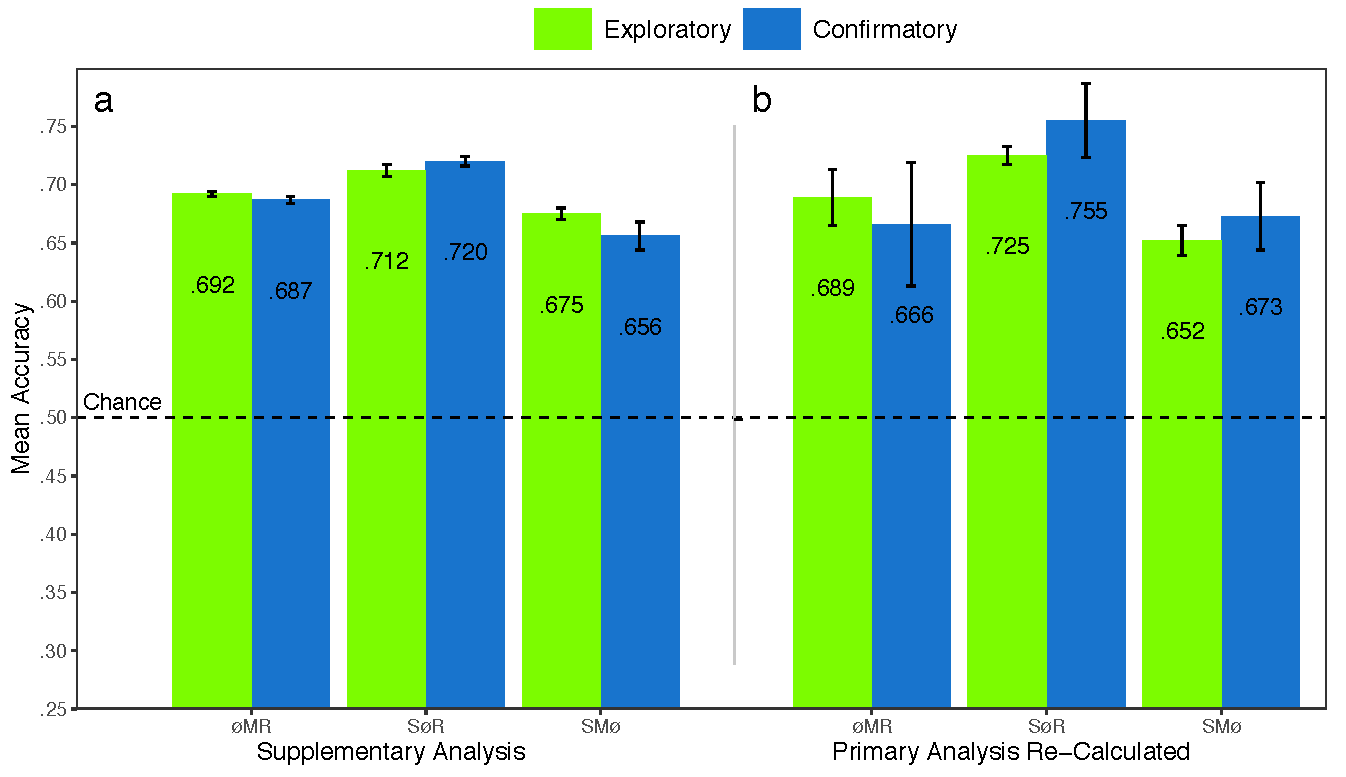
\includegraphics{figures/supp_analysis/supp_subset_chance.pdf}
\caption{\label{fig:supp-chance}The graph represents the average accuracy reported for each subset of the Exploratory and Confirmatory timeline data for (a) the supplementary analysis, and the (b) re-calculated accuracies from the primary analysis. All of the data subsets were decoded at levels better than chance (.50). The error bars represent standard errors.}
\end{figure}

\begin{table}[!h]
    \centering
    \caption{Supplementary Subset Comparisons}
    \label{tab:supp-comparisons}
    \begin{tabular}{l c c c c}
         & \multicolumn{2}{c}{Exploratory} & \multicolumn{2}{c}{Confirmatory} \\
        \hline
        Comparison & \textit{t} & \multicolumn{1}{c|}{\textit{p}} & \textit{t} & \textit{p} \\
        \hline
        $\varnothing$MR vs. S$\varnothing$R & 3.248 & \multicolumn{1}{c|}{.008} & 3.094 & .012 \\
        $\varnothing$MR vs. SM$\varnothing$ & 2.875 & \multicolumn{1}{c|}{.021} & 2.923 & .018 \\
        S$\varnothing$R vs. SM$\varnothing$ & 6.123 & \multicolumn{1}{c|}{< .001} & 6.017 & < .001 \\
        \hline
    \end{tabular}
\end{table}

\begin{figure}
\centering
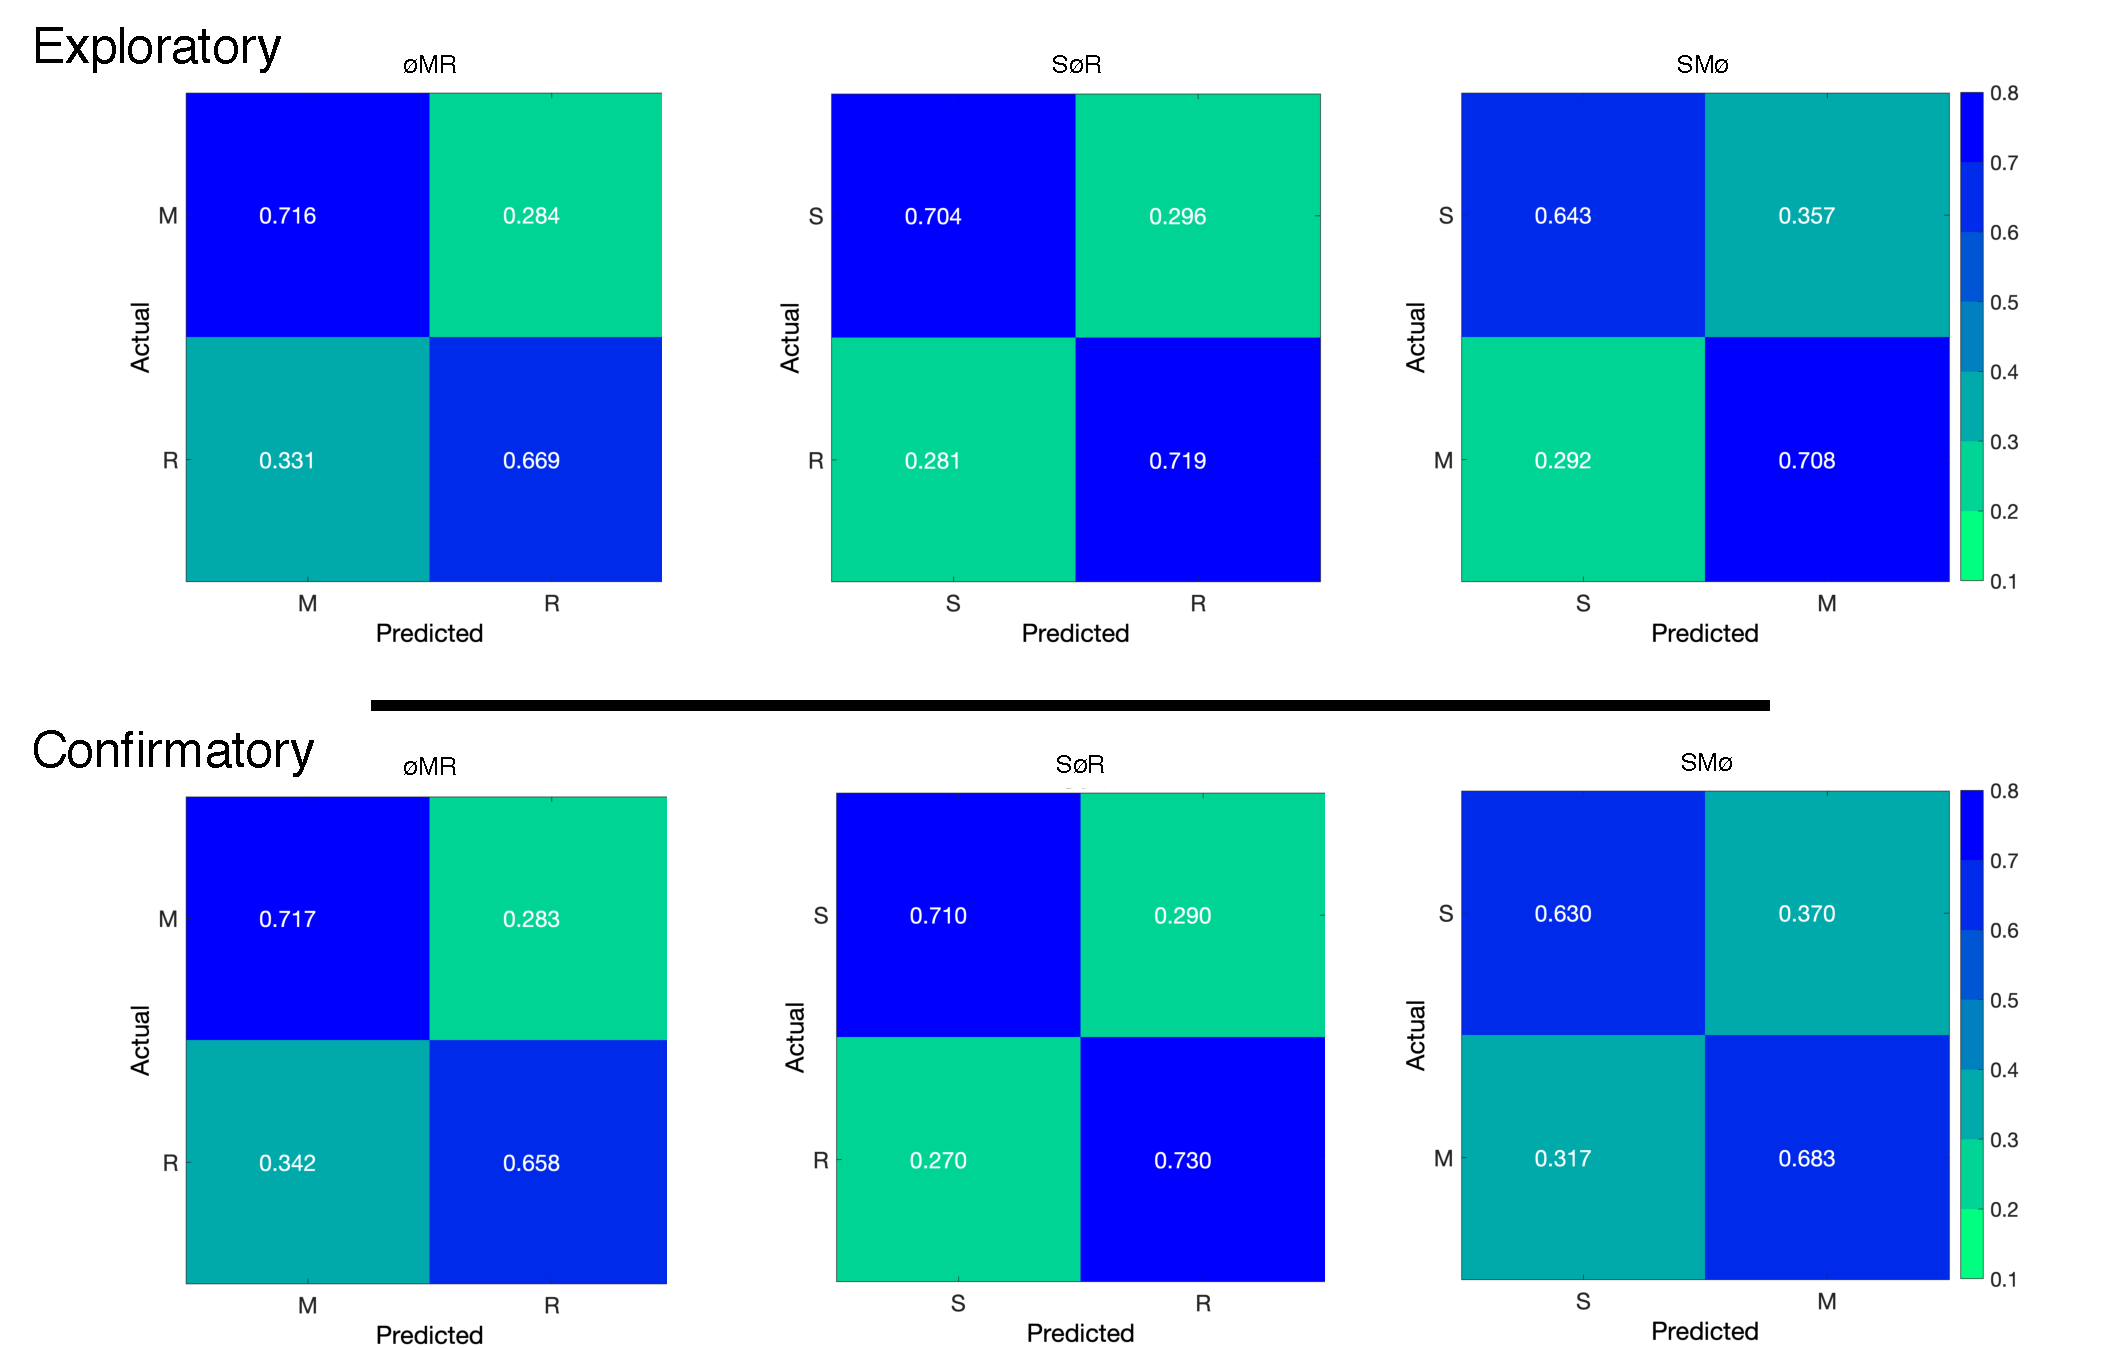
\includegraphics{figures/supp_analysis/confusion_matrices/supp_conf_matrices.pdf}
\caption{\label{fig:supp-conf-matrices}The confusion matrices represent the average classification accuracies for each condition of the timeline data (S = Search, M = Memorize, R = Rate). The vertical axis of the confusion matrices represents the actual condition for the trial. The horizontal axis of the confusion matrices represents the condition that was predicted by the model.}
\end{figure}

The accuracies for all of the data subsets observed in the supplementary analysis were higher than the accuracies observed in the main analysis. Although there is a clear difference in accuracy, the primary analysis was classifying three categories (chance = .33) and the supplementary analysis was classifying two categories (chance = .50). Because the baseline chance performance was different for the primary and supplemental analyses, any conclusions drawn from a comparison of the results of analyses could be misleading. For this reason, we revisited the results from the primary analysis and re-calculated the predictions to be equivalent to a 50\% chance threshold. Because the cross-validation scheme implemented by the DeLINEATE toolbox (\url{http://delineate.it}; Kuntzelman et al., \textcolor{red}{in press}) guaranteed an equal number of trials in the test set were assigned to each condition for each dataset, we were able to re-calculate 2-category predictions from the 3-category predictions presented in the confusion matrices from the primary analysis (see Figure \ref{fig:timeline-conf-matrices}). The predictions were re-calculated using the following formula: Prediction\(_{(A, A, A\varnothing C)}\) = Prediction\(_{(A, A, ABC)}\) / (Prediction\(_{(A, A, ABC)}\) + Prediction\(_{(A, C, ABC)}\)). For example, accuracy for the Search classification for S\(\varnothing\)R would be calculated with the following: Prediction\(_{(S, S, S\varnothing R)}\) = Prediction\(_{(S, S, SMR)}\) / (Prediction\(_{(S, S, SMR)}\) + Prediction\(_{(S, R, SMR)}\), where Prediction\(_{(S, R, S\varnothing R)}\) is the ratio of Search trials that were misclassified as Rate.

The results for the re-calculated predictions followed a pattern similar to the main supplementary analysis (see Figure \ref{fig:supp-chance}b). Looking back at the primary analysis, the 3-category classifications predicted the Memorize conditions with the lowest accuracy (c.f., Search and Rate conditions), and mis-classifications of the Search and Rate conditions were most often categorized as Memorize (see Figure \ref{fig:timeline-conf-matrices}). Because the Memorize condition was mis-classified more often than the other conditions in the primary analysis, the removal of the third class in the re-calculated SM\(\varnothing\) and \(\varnothing\)MR subsets resulted in a disproportionate amount of mis-classified Memorize trials being removed from those data subsets, somewhat eliminating the tendency to mis-classify Search and Rate trials as Memorize (see Figure \ref{fig:recalc-conf-matrices}). Nevertheless, the re-calculated SM\(\varnothing\) and \(\varnothing\)MR subsets were classified less accurately than S\(\varnothing\)R, just as in the main supplementary analysis.

\begin{figure}
\centering
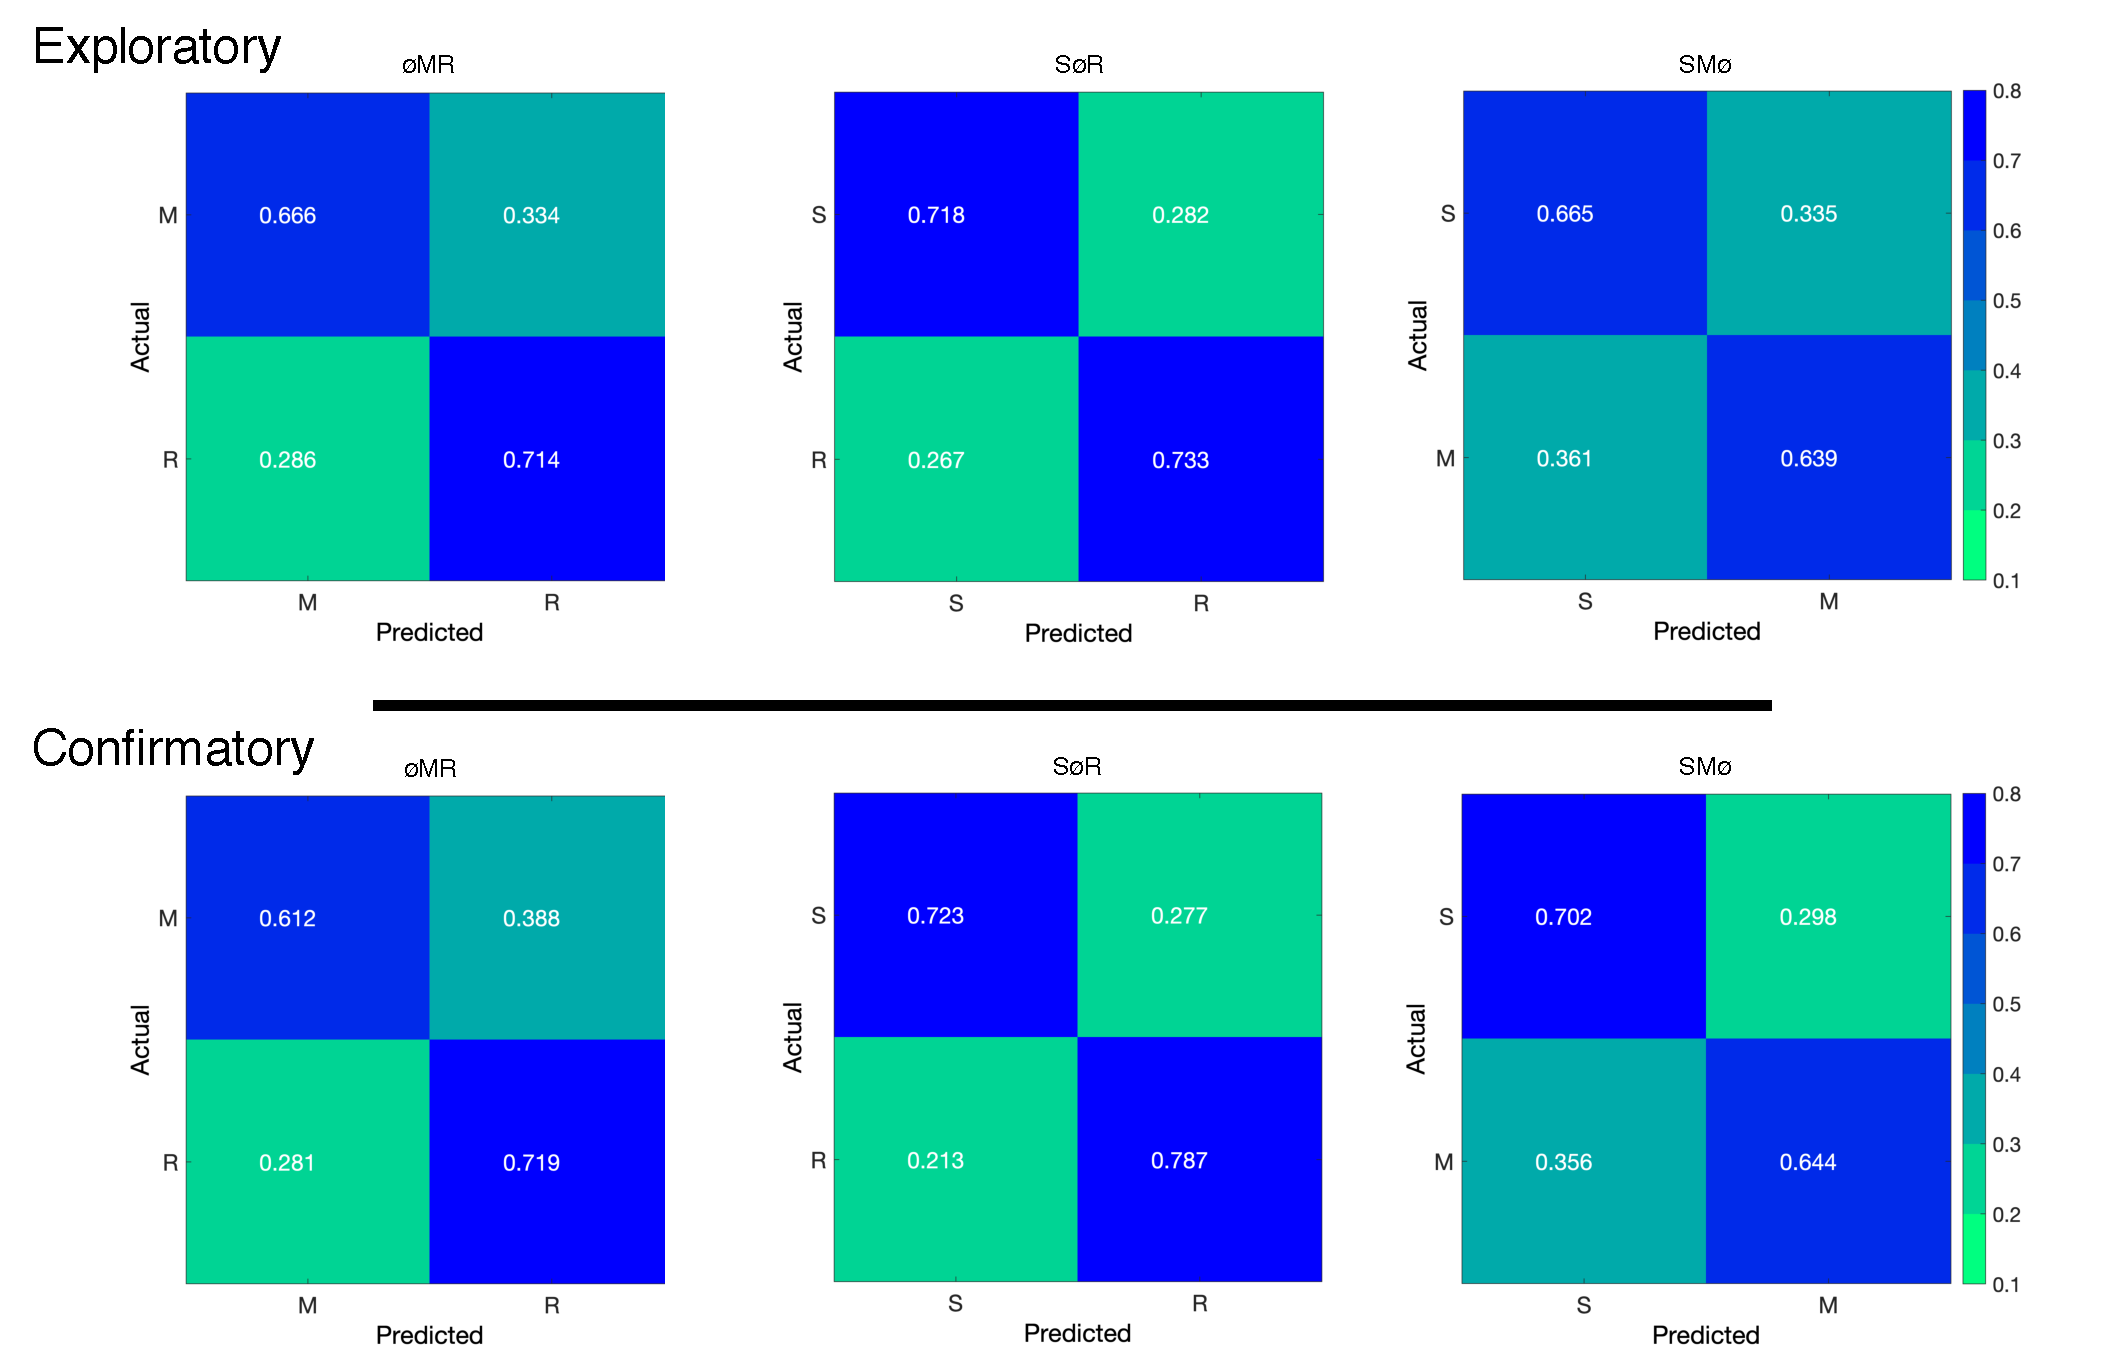
\includegraphics{figures/supp_analysis/recalculations/confusion_matrices/recalc_conf_matrices.pdf}
\caption{\label{fig:recalc-conf-matrices}The confusion matrices represent a re-calculation of the classification accuracies for each category from the primary analysis. This re-calculation is meant to make the accuracies presented in the primary analysis (chance = .33) equivalent to the classification accuracies presented in the supplementary analysis (chance = .50).}
\end{figure}


\end{document}
